\chapter{Lagrangian Domain: Vortex Particle Method}
\label{ch:lagrangian}

	
%	\lsymb[f]{$\mathbf{x}$}{Position vector}{\si{\m}}{x}
%	\lsymb[f]{$\mathbf{x}_p$}{Position vector of the particle}{\si{\m}}{xp}
%	\lsymb[f]{$\mathbf{x}_{\nu}$}{Position vector of particle to be diffused}{\si{\m}}{xmm}
%	\lsymb[f]{$t$}{Time}{\si{\s}}{t}
%	\lsymb[f]{$\mathbf{u}$}{Velocity}{\si{\m\per\s}}{u}
%	%\lsymb[f]{$\mathbf{u}\left(\mathbf{x},t\right)$}{Velocity field}{$[m\cdot s^{-1}]$}{ua}
%	\lsymb[f]{$p$}{Pressure}{\si{\pascal}}{p}
%	\lsymb[f]{$\mathbf{u}^h$}{Discrete velocity}{\si{\m\per\s}}{uh}	
%	\lsymb[f]{$\mathbf{u}_{\infty}$}{Free-stream velocity}{\si{\m\per\s}}{ul}
%	\lsymb[f]{$\mathbf{u}_{\omega}$}{Vortical velocity}{\si{\m\per\s}}{uz}
%	\lsymb[f]{$\mathbf{u}_{\phi}$}{Potential velocity}{\si{\m\per\s}}{up}
%	\lsymb[f]{$\mathbf{u}_{\gamma}$}{Vortex sheet induced velocity}{\si{\m\per\s}}{uc}
%	\lsymb[f]{$\mathbf{u}_{\mathrm{ext}}$}{External induced velocity}{\si{\m\per\s}}{ue}
%	\lsymb[f]{$\mathbf{u}_{b}$}{Velocity of the body}{\si{\m\per\s}}{ub}	
%	\lsymb[f]{$\mathbf{u}_{\mathrm{slip}}$}{Boundary slip velocity}{\si{\m\per\s}}{us}	
%	\lsymb[f]{$u_{r}$}{Radial velocity}{\si{\m\per\s}}{ur}	
%	\lsymb[f]{$u_{\theta}$}{Angular velocity}{\si{\m\per\s}}{uhh}	
%
%		
%	\lsymb[f]{$N_p$}{Number of particles}{-}{np}	
%	\lsymb[f]{$\mathbf{K}$}{Biot-Savart kernel}{-}{k}
%	\lsymb[f]{$\mathbf{K_{\sigma}}$}{Vortex blob kernel}{-}{kb}	
%	\lsymb[f]{$h$}{Nominal particle spacing}{\si{m}}{h}	
%	\lsymb[f]{$\mathrm{overlap}$}{Overlap ratio of the blobs}{-}{o}	
%	\lsymb[f]{$W$}{Interpolation kernel weight}{-}{w}
%	\lsymb[f]{$\mathcal{E}$}{Enstrophy}{\si{m^2.s^{-2}}}{en}
%	\lsymb[f]{$c^2$}{Diffusion parameter}{-}{c}
%	\lsymb[f]{$\mathbf{\hat{n}}$}{Normal vector}{-}{n}
%	\lsymb[f]{$\mathbf{\hat{s}}$}{Tangent vector}{-}{s}	
%	\lsymb[f]{$h_{\nu}$}{Characteristic diffusion distance}{\si{m}}{hm}		
%	\lsymb[f]{$k_{d}$}{Diffusion frequency multiple}{-}{kd}			
%	
%	\lsymb[f]{$\mathbf{A}$}{Vortex panel influence matrix}{-}{kd}				
%
%	\lsymb[f]{$r$}{Radial position}{\si{m}}{r}
%
%	\gsymb[f]{$\zeta_{\sigma}$}{Smooth cut-off function of the blob}{-}{ff}	
%	\gsymb[f]{$\rho$}{Density}{\si{kg.m^{-3}}}{qq}
%	\gsymb[f]{$\nu$}{Kinematic viscosity}{\si{m^2.s^{-1}}}{mm}
%	\gsymb[f]{$\Gamma$}{Circulation}{\si{m^2.s^{-1}}}{c}
%	\gsymb[f]{$\Gamma_{\omega}$}{Circulation of the fluid}{\si{m^2.s^{-1}}}{cxx}	
%	\gsymb[f]{$\Gamma_{\gamma}$}{Circulation of vortex sheet}{\si{m^2.s^{-1}}}{ccc}		
%	\gsymb[f]{$\Gamma_{b}$}{Circulation of moving body}{\si{m^2.s^{-1}}}{cb}			
%	\gsymb[f]{$\omega$}{Vorticity}{\si{s^{-1}}}{xx}
%	\gsymb[f]{$\omega^h$}{Discrete vorticity field}{\si{s^{-1}}}{xxh}
%	\gsymb[f]{$\alpha_p$}{Circulation of the particle}{\si{m^2.s^{-1}}}{aap}
%	\gsymb[f]{$\beta_p$}{Corrected circulation of the particle}{\si{m^2.s^{-1}}}{bbp}
%	%\gsymb[f]{$\epsilon$}{Distance between the particles}{$[m]$}{eep}
%	\gsymb[f]{$\sigma$}{Core size}{\si{m}}{rr}
%	\gsymb[f]{$\Delta t_d$}{Diffusion time-step size}{\si{s}}{dtd}	
%	\gsymb[f]{$\Delta t_c$}{Convection time-step size}{\si{s}}{dtc}		
%	\gsymb[f]{$\gamma$}{Vortex sheet strengths}{\si{s}}{cc}		
%	\gsymb[f]{$\xi$}{Scale relative position of particle to stencil node}{-}{nn}
%	\gsymb[f]{$\epsilon$}{Relative error}{-}{ee}
%	\gsymb[f]{$\tau$}{Scaled viscous time}{\si{m^2}}{ss}
%	\gsymb[f]{$\Gamma_c$}{Circulation of the vortex core}{\si{m^2.s^{-1}}}{cc}

%To model the flow around a VAWT, several approaches can be taken, Vermeer at al. (2003) \cite{Vermeer2003} have also summarized in their paper. The two main approaches of investigating the flow is either employing a numerical method to simulate the flow or through experimental simulations.

%Leishman (2006) \cite{leishman2006principles} has shown that there are several simplified, efficient numerical tools that can be used to model the performance of a VAWT. Methods such as actuator disk theory and blade element momentum theory and deals with simplified Navier-Stokes equations and is very useful to evaluate the trend of certain design parameter. However, as they are highly simplified, complex flow phenomenons that has severe impact of the performance characteristics of the VAWT such as flow separation during dynamic stall, vortex shedding during the rotation and blade-wake interaction cannot be simulated. In order to understand them, either experimental investigation such as in wind tunnel or full Navier-Stokes simulations have to undertaken. So to understand the flow behaviour of a VAWT, several numerical research have been performed \cite{Almohammadi2013} \cite{Ferreira2007} \cite{Islam2008} \cite{Merz2012} and experimental researches by Ferreira \cite{SimaoFerreira2008} \cite{Ferreira} and others \cite{Howell2010} \cite{Mertens2003}.
%\index{Actuator disk}

%All the numerical method that was grid-based struggled with dealing with large number of mesh cells for high Reynolds numbers and the numerical method that employed simplified Navier-Stokes methods had to sacrifices some accuracies.The experimental investigation also come with drawbacks as they are require more financial resources and usually only feasible to model the scaled VAWTs.

%This is the main relevance of the hybrid vortex particle method for the VAWT investigations. By utilizing the two methods together, the vortex particle method away from body, and Navier-Stokes solver with turbulence model in the near-body region, one will be able to tackle the challenges in an efficient manner.

%Therefore, this chapter is dedicated to given an overview on the theory of the Vortex Particle Method which we will employ with coupled Navier-Stokes solver. 

%------------------------------------------------------------------------------------------------------
%------------------------------------------------------------------------------------------------------
%------------------------------------------------------------------------------------------------------
\section{Introduction to the Vortex Particle Method}
\indexAcron{Vortex Particle Method}{VPM} is a numerical method employed in of computational fluid dynamics that deals with the evolution of the vorticity of the fluid in a Lagrangian description. In an Eulerian formulation, the fluid is viewed at a fixed window where the change in the fluid properties are evaluated. However, the Lagrangian formulation, regards the fluid as a collection of particles (or elements) carrying properties of the fluid (vorticity, mass, etc.). 

Efficient discretization of the fluid domain becomes a difficult task for cases such as \printAcron{Vertical-Axis Wind Turbine}{VAWT}, where the wake geometry is usually unknown and highly unsteady. Discretizing such wake using Eulerian formulation usually becomes inefficient unless one manually adapts the mesh geometry over time. This is one of the advantage of the VPM. The VPM only needs fluid elements where there is vorticity meaning that the method is inherently auto-adaptive when discretizing the fluid domain. Furthermore, with computational acceleration methods such as \printAcron{Fast-Multipole Method}{FMM} and parallel computation in \printAcron{Graphics Processing Units}{GPU} enables an efficient evolution of the vorticity wake. However, the key advantage of the VPM is that it is ideal for capturing the resolving the long-time characteristics of the unsteady compact vortical structures that are shed off from the VAWT blades \cite{Stock2010a}.

The advantage of the Lagrangian vortex method w.r.t the Eulerian method was summarized by Wee and Ghoniem \cite{Wee2006a}:
\begin{itemize}
\item Eulerian methods introduce dissipation, even in flows with zero velocity gradient. However such error as minimized at the convection of the Lagrangian method.
\item The numerical stability is not restricted by the CFL condition.
\item The support of the Lagrangian elements are a small fraction of the fluid domain. The support is confined to location of non-zero vorticity, making the method naturally grid adaptive.
\end{itemize}

The main literature on the VPM (the Lagrangian domain of the hybrid method), is the book of Cottet and Koumoutsakos, Vortex Methods: Theory and Practice \cite{Cottet2000a}. It gives an insight on the fundamentals of the vortex method (specifically VPM) and gives a summary on hybrid methods.

\subsection{Vorticity}
The vorticity $\omega$, the governing element of the VPM. It is given by
	\begin{equation}
	\mathbf{\omega} = \nabla \times \mathbf{u},
	\label{eq:lag_vort}
	\end{equation}
where $\mathbf{u}$ is the velocity vector field. The circulation $\Gamma$ is defined by Stokes' theorem,

	\begin{equation}
	\Gamma = \int_L\mathbf{u}\cdot \mathrm{d}s= \int_A (\nabla \times u) \cdot \mathbf{n}\ \mathrm{d}A = \int_A\omega\cdot\mathbf{n}\ \mathrm{d}A,
	\label{eq:definitionOfCirculation}
	\end{equation}

and represents the flux integral of vorticity across the surface $A$, having the line $s$ as boundary. Figure \ref{fig:vorticityCirculation} depicts the relation with velocity $\mathbf{u}$, vorticity $\omega$ and the circulation $\Gamma$ in an arbitrary domain.

	\begin{figure}[!h]
	\centering
	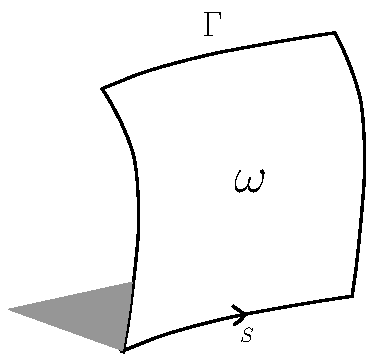
\includegraphics[width=0.3\linewidth]{./figures/lagrangian/vorticityCirculation_updated.pdf}
	\caption{Definition of the circulation in the fluid.}
	\label{fig:vorticityCirculation}
	\end{figure}

 
\subsection{Velocity-Vorticity formulation of the Navier-Stokes equations}
The governing equation of the vortex particle method is the velocity-vorticity formulation $\mathbf{u}-\omega$ of the Navier-Stokes equations \cite{Cottet2000a}. The 2-D incompressible Navier-Stokes momentum equation is given as,
	\begin{equation}
	\frac{\partial \mathbf{u}}{\partial t} + \mathbf{u}\cdot\nabla\mathbf{u} = - \frac{1}{\rho} \nabla p + \nu \nabla^2\mathbf{u},
	\label{eq:mom}
	\end{equation}
relating the velocity field $\mathbf{u}\left(\mathbf{x},t\right)$ to the pressure field $p\left(\mathbf{x},t\right)$, the kinematic viscosity $\nu$ and density $\rho$. Furthermore, the incompressibility constraint given as,
	\begin{equation}
	\nabla\cdot\mathbf{u} = 0,
	\label{eq:la_ic}
	\end{equation}
must also be satisfied. To obtain the velocity-vorticity formulation, we should take the curl of equation \ref{eq:mom}, 
	\begin{equation}
	\frac{\partial \omega}{\partial t} + \mathbf{u}\cdot\nabla\omega = \nu \nabla^2 \omega,
	\end{equation}
which only relates the vorticity to the velocity enabling us to remove the pressure term. Note that as we are dealing with 2D flows, 3D terms (such as the stretching term) does not appear.

\subsection{Viscous splitting algorithm}
The VPM was initially used to model the evolution of incompressible, inviscid flows. However, in order to simulate a real flow, we must also deal with the viscous behavior of the fluid. Chorin in 1973 \cite{Chorin1973a}, showed that using the viscous splitting algorithm, it is possible to take the viscous effects of the flow into account. 

The viscous splitting algorithm is a fractional step method, where the viscous and the inviscid part of the vorticity transport equation are dealt with in two subsequent sub-steps, 

	\begin{enumerate}
	\item \textbf{Convection} (sub-step 1):
		\begin{equation}
		\frac{\partial\omega}{\partial t} + \mathbf{u}\cdot\nabla\omega=0;
		\label{eq:convectionEulerian}
		\end{equation}
		
	\item \textbf{Diffusion} (sub-step 2):
		\begin{equation}
		\frac{\partial\omega}{\partial t} = \nu\nabla^2\omega.
		\label{eq:vsa2}
		\end{equation}
	\end{enumerate}

The first sub-step of the evolution deals with the convection of vorticity. The diffusion of vorticity field is dealt with in the second sub-step. There are several advantages to this type of evolution. As the convection and diffusion are handled separately, there is minimum dissipation during the convection step and furthermore, there is no restriction of the advection CFL number, see Wee (2006) \cite{Wee2006a}.

There are many ways of treating the diffusion of the vorticity field. In this work, we initially used the modified interpolation kernel by Wee (2006) \cite{Wee2006a} that simultaneously discretizes diffusion and redistributes the vortex particles. Later, we used a simple redistribution scheme of Tutty (2010) \cite{Tutty2010a}, that did not constraint the minimum time-step size, see section \ref{sec:diffusionVM}.

%------------------------------------------------------------------------------------------------------
%------------------------------------------------------------------------------------------------------
%------------------------------------------------------------------------------------------------------
\section{Spatial Discretization: Generation of Vortex Blobs}
\label{sec:spatialDiscretization}

The particle in the Vortex Particle Method arises from the discretization of the vorticity field, equation \ref{eq:lag_vort}. 

\subsection{Discrete form of vorticity field}
\label{subsec:discreteVorticity}
The vorticity field is discretized using $N$ vortex particles. The discrete vorticity field is given as,
	\begin{equation}
	\omega\left(\mathbf{x},t\right) \simeq \omega^h\left(\mathbf{x},t\right) = \sum_{p}\alpha_p\left(t\right)\delta \left[\mathbf{x}-\mathbf{x}_p\left(t\right)\right],
	\end{equation}
where $\delta$ is the Dirac delta function, $\alpha_{p}$ is the circulation carried by the particle at $\mathbf{x}_p$. We must note that $\omega^h$ is the discrete vorticity field and therefore in an approximation of the continuous vorticity field $\omega$. 

\subsection{Biot-Savart Law}
A velocity field $\mathbf{u}$ that satisfies the incompressibility constraint, equation \ref{eq:la_ic}, can be decomposed using the Helmholtz decomposition,
	\begin{equation}
	\mathbf{u} = \mathbf{u}_{\omega} + \mathbf{u}_{\phi},
	\label{eq:helmholtz}
	\end{equation}
where $\mathbf{u}_{\omega}$ is the rotational component of the velocity and $\mathbf{u}_{\phi}$ is the irrotational component, i.e. the solenoidal and the potential velocity respectively. The irrotational component is equal to the free-stream velocity $\mathbf{u}_{\infty}$ for an incompressible, unbounded flows. Whereas for bounded flows, we must include the presence of the body as the full Helmholtz decomposition becomes,
\begin{equation}
\mathbf{u} = \mathbf{u}_{\omega} + \mathbf{u}_{\phi} + \mathbf{u}_{b},
\end{equation}
where $\mathbf{u}_b$ is the velocity due to the body, see section \ref{sec:boundaryConditions}. The velocity can be related to the vorticity using the Biot-Savart law given as,
	\begin{equation}
	\mathbf{u}_{\omega} = \mathbf{K}\star\omega,
	\end{equation}
where $\star$ is the convolution of the vorticity with the 2-D Biot-Savart kernel $\mathbf{K}$ given by,
	\begin{equation}
	\mathbf{K} = \frac{1}{2\pi\left|\mathbf{x}\right|^2}\left(-x_2,x_1\right).
	\label{eq:GreensKernel}
	\end{equation}
From the kernel, we see that as the distance to the kernel center approaches zero ($\mathbf{x} \rightarrow 0$), the kernel goes to infinity. The singularity of the kernel $\mathbf{K}$ is removed by mollifying the kernel distribution ensuring smooth velocity distribution.

%Thus the discrete vorticity field is an $N$-body problem inducing velocity on each other. So, to evolve the vorticity field, we simply have to evolve the vortex particles with the induced velocity acting on it. This is the main advantage of the vortex particle method as there are efficient methods to evaluate the induced velocities. The $N$-body problem can be parallelized in GPUs, and furthermore the induced velocity calculations can be simplified using fast summation methods such as the \printAcron{Fast Multipole Method}{FMM}, reducing the problem from $\mathcal{O}(N^2)$ to $\mathcal{O}(N)$, in an ideal case.


\subsection{Mollified vortex kernels}

A mollified vortex particle is called the vortex blob having a non-zero vortex core size $\sigma$. A smoothing function $\zeta$ is used to mollify the kernel $\mathbf{K}$, satisfying the constraint $\int \zeta = 1$, such that the circulation is conserved. An ideal choice for a smoothing function is the Gaussian distribution, given as,
	\begin{equation}
	\zeta_{\sigma} = \frac{1}{k\pi\sigma^2}\exp\left(-\frac{\left|\mathbf{x}\right|}{k\sigma^2}\right),
	\end{equation}

where typically $k$ is either 1, 2 or 4 and determines the width of the kernel, with $\sigma$ being the core-size of the vortex blob. Figure \ref{fig:gaussianDistribution} depicts the smoothing function $\zeta_{\sigma}$ with $k=2$ and $\sigma = 1$, decaying quickly away from the center of the core. The mollified Biot-Savart kernel $\mathbf{K}_{\sigma}$ is given as,	 
	\begin{equation}
	\mathbf{K}_{\sigma} = \mathbf{K} \star \zeta_{\sigma}, 
	\end{equation}

	\begin{figure}[t]
	\centering
	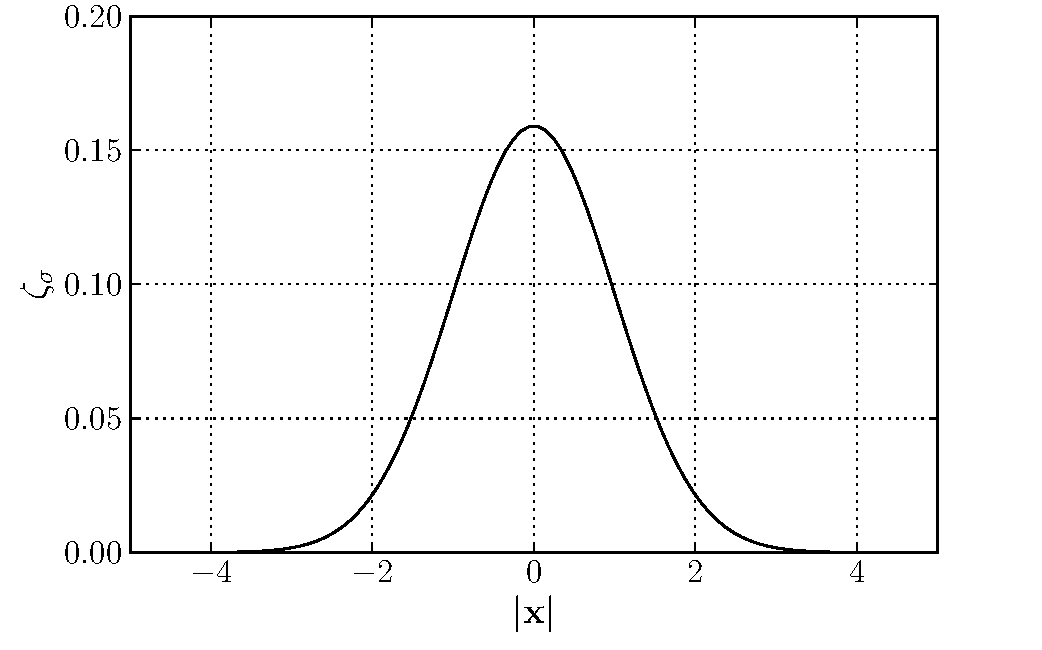
\includegraphics[width=0.7\textwidth]{figures/lagrangian/gaussianKernel.pdf}
	\caption{The smoothing function $\zeta_{\sigma}$ for a gaussian distribution with $k=2$, $\sigma=1$.}
	\label{fig:gaussianDistribution}
	\end{figure}

giving us the discrete mollified vorticity field as,
	\begin{equation}
	\omega^h\left(\mathbf{x},t\right) = \sum_p \alpha_p\left(t\right)\zeta_{\sigma}\left[\mathbf{x}-\mathbf{x}_p\left(t\right)\right],
	\label{eq:mollifiedVorticityField}
	\end{equation}
and the discrete mollified velocity field as,
	\begin{equation}
	\mathbf{u}^h\left(\mathbf{x},t\right) = \sum_p \mathbf{K}_{\sigma}\left[\mathbf{x}-\mathbf{x}_p\left(t\right)\right]\alpha_p\left(t\right).
	\end{equation}

Koumoutsakos and Chorin \cite{Cottet2000a}, explained that in order to ensure the smoothness of the velocity field, the vortex blobs need to have an overlap with each other. The overlap ratio $Ov$ is defined as,
	\begin{equation}
	\mathrm{Ov} = \frac{\sigma}{h},
	\label{eq:overlapRatio}
	\end{equation}
where $h$ is the nominal particle spacing, and $\sigma$ is the vortex blob core size. Figure \ref{fig:blobOverlap} shows the visual representation of this definition. 

The overlap constraint is violated during the convection of the vortex blobs. Due to the strains in the flow, the vortex blobs cluster together at certain region and disperse at others. This localized clustering effect is seen as a Lagrangian grid distortion, which is dealt with using a remeshing technique, section \ref{subsec:remeshing}.

	\begin{figure}[!t]
	\centering
	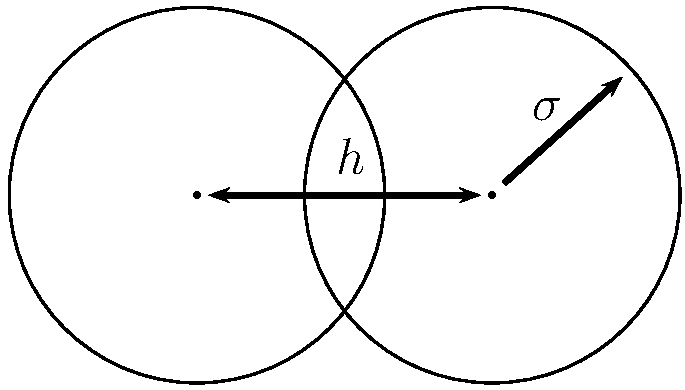
\includegraphics[width=0.4\textwidth]{figures/lagrangian/blobOverlap.pdf}
	\caption{Vortex blob with an overlap $Ov = \sigma/h$}
	\label{fig:blobOverlap}
	\end{figure}

\subsection{Vortex blob initialization}
\label{subsec:vortexBlobInitialization}
Now the question arises on how should we initialize the particle's circulation strengths $\alpha_p$. The common approach that is used as a standard is to estimate the particles strength by the local properties,
	\begin{equation}
	\alpha_p = \omega_p\cdot h^2,
	\label{eq:particleCirculationAssignment}
	\end{equation}

	\begin{figure}[!b]
	\centering
	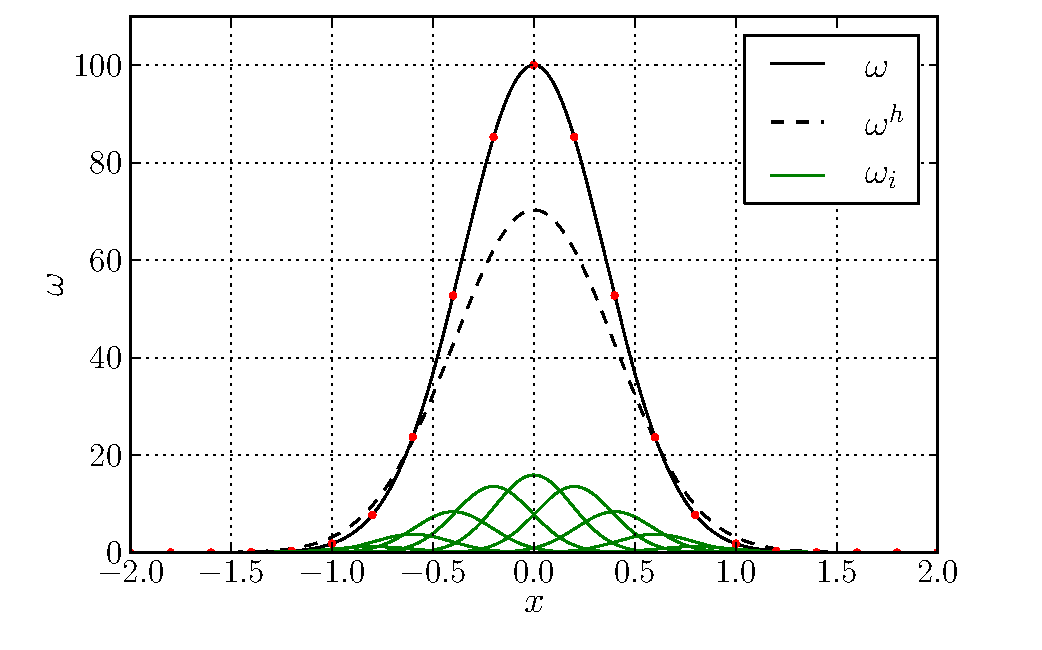
\includegraphics[width=0.7\textwidth]{figures/lagrangian/particleInitialization.pdf}
	\caption{Mollified vorticity field of a gaussian vorticity distribution with $\mathrm{overlap}=1.0$, $\sigma=0.19$, and $h=0.19$. Vortex blob strengths was assigned using equation \ref{eq:particleCirculationAssignment}, sampling the exact vorticity [{\color{plotRed}{$\bullet$}}, red dot]. Figure depicts the exact vorticity distribution $\omega$ [---, solid black], vorticity distribution of each blob $\omega_i$ [{\color{darkgreen}{---}}, dashed green], and the mollified vorticity field from the blobs $\omega^h$ [- -, dashed black].  }
	\label{fig:particleInitialization}
	\end{figure}

meaning that the particle carry the circulation of its local area. This might seem like a valid assumption as the circulation of a given area is the integral of the vorticity in the area, given by equation\ \ref{eq:definitionOfCirculation}, and therefore we will be conserving the circulation as all the circulation in the fluid is represented by the blobs.

However, this type of initialization suffers some accuracy in the vorticity field itself as the vorticity field represented by the blobs is no longer the initial vorticity field, but the mollified vorticity field, equation \ref{eq:mollifiedVorticityField}. Barba and Rossi \cite{Barba2010a}, has described this problem as gaussian blurring of the original vorticity field. Even though the particle have acquired the correct circulation strengths (i.e the local property), when evaluating the mollified vorticity field, we see that there is a mismatch with the original vorticity field, figure \ref{fig:particleInitialization}. 

Another way of viewing this phenomenon is to say that the conservation of circulation is only valid globally (for an infinite domain), but once we try to conserve circulation locally (e.g. in a given sub-domain), is does not satisfy anymore. Figure \ref{fig:particleInitialization} shows this effect for a simple gaussian initial vorticity distribution $\omega$. The mollified vorticity field is given as $\omega^h$ and even though the integral of both function is the same (conservation of circulation is satisfied), the vorticity functions do not match. This is does not cause a lot of issues when we only dealing with vortex particle method, however once we start using domain decomposition methods, this problem is an issue. As the vorticity is the communication between both methods, we must have accurate vorticity distribution.

A common strategy, used by Koumoutsakos, Cottet, and other for recovering the initial vorticity field is to perform the Beale's method \cite{Beale1988} \cite{Cottet2000a}.


\subsubsection*{Beale's Iterative Method}
\label{subsubsec:BealesMethod}
The Beale's method is particle circulation processing scheme where the circulation of the particles are modified such that the mollified vorticity field matches the indented vorticity field (the initial vorticity field). The recovery of the vorticity field is done by performing a discrete deconvolution,
	\begin{equation}
	\sum_j^N \beta_j \zeta_{\sigma}\left(\mathbf{x}_i-\mathbf{x}_j\right) = \omega_i,
		\end{equation}
where $\beta_j$ is the circulation of the particles at positions $\mathbf{x}_j$ such that it matches the exact vorticity $\omega_i$ at the position $\mathbf{x}_i$ that we are evaluating.  As we are try to solve for a $N$ unknown problem, we must set up an $N$ system of equations. Multiplying both sides with the area associated to the blobs, we get
	\begin{equation}
	\mathbf{A}_{ij} \beta_j = \alpha_i^{\mathrm{exact}},
	\end{equation}
where
	\begin{equation}
	\mathbf{A}_{ij} = \zeta_{\sigma}\left(\mathbf{x}_i - \mathbf{x}_j\right) \cdot h^2.
	\end{equation}

This is an $N \times N$ matrix containing the weights of the influence of each particle on each other. When we are dealing with large number of vortex blobs, we see that it is very expensive to invert the matrix $\mathbf{A}$, meaning that we would have to use a more efficient method. Furthermore as the deconvolution problem is a severely ill-condition problem \cite{Cottet2000a}, we should not directly invert the matrix. Beale's proposition to this problem was to iteratively solve for the solution,
	\begin{equation}
	\beta_{j}^{n+1} = \alpha_i + \beta_i^n - \mathbf{A}_{ij}\cdot\beta_j^n
	\end{equation}
	
We see that with just two iterations, the error between the mollified and exact vorticity field reduces drastically, figure \ref{fig:bealesCorrection}. Koumoutsakos and Cottet \cite{Cottet2000a}, had shown that there was a drastic improvement in the velocity with just two to three iterations. However, the average vorticity of the blobs cell $\tilde{\omega} = \beta/h^2$ (red dot in figure \ref{fig:bealesCorrection}), is more peaky and no longer matches the initial vorticity distribution. This means that if we try to fix the mollified vorticity distribution to match the correct initial vorticity distribution, we corrupt the local circulation even more.

The another downside of using the Beale's correction method that it is only valid for an infinite domain as it performs a discrete deconvolution of a gaussian kernel with an infinite span. Therefore it applies to all of the fluid domain, meaning that if we are dealing with a decomposed domain with finite bounds, the Beale's correction cannot be used and would result in spurious results. So the Beale's correction can and should only be used for correcting the vorticity field of the whole fluid domain.

	\begin{figure}[t]
	\centering
	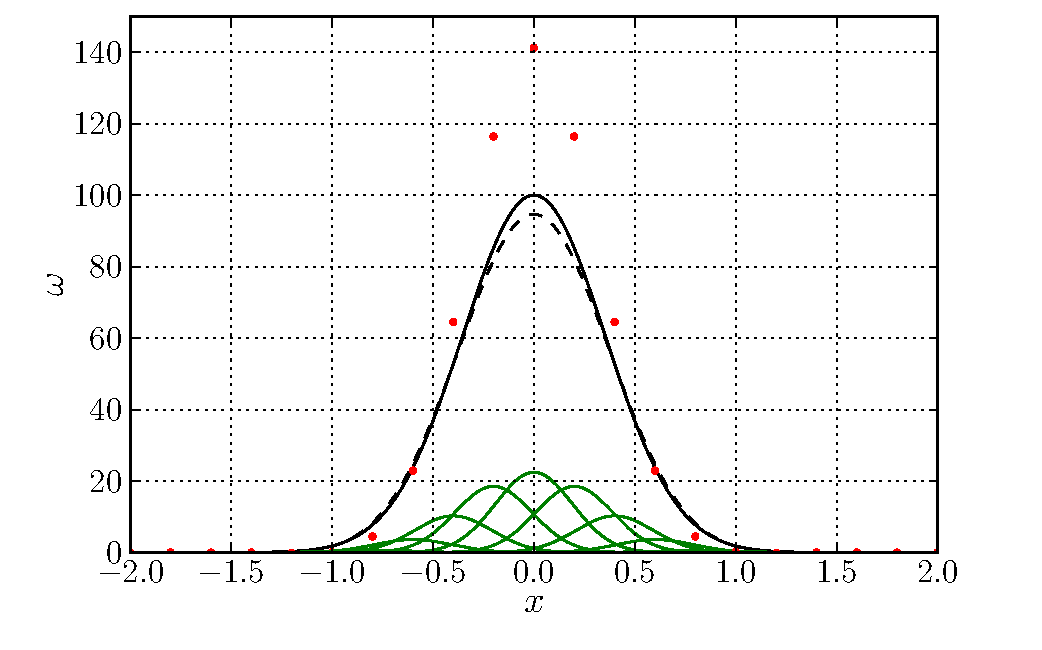
\includegraphics[width=0.7\textwidth]{figures/lagrangian/bealesCorrection.pdf}
	\caption{Mollified vorticity field after two Beale's iteration, with $\mathrm{overlap}=1.0$, $\sigma=0.19$, $h=0.19$. Figure depicts exact vorticity distribution $\omega$ [---, solid black], vorticity distribution of each blob $\omega_i$ [{\color{plotGreen}{---}}, dashed green], the mollified vorticity field $\omega^h$ [- -, dashed black], and the corrected blob cell vorticity $\tilde{\omega}=\beta/h^2$ [{\color{plotRed}{$\bullet$}}, red dot].}
	\label{fig:bealesCorrection}
	\end{figure}

\subsubsection{Convergence of particle discretization}
\label{subsubsec:convergenceInterpolation}
An alternate method to reduce the gaussian blurring of the vorticity field is to reduce the overlap (i.e. increase the overlap number) of the vortex blobs, and also increase the spatial resolution. This approach does not solve the gaussian blurring problem, but only minimizes its effect.
	
\begin{figure}[t]
        \centering
        \begin{subfigure}[b]{0.5\textwidth}
                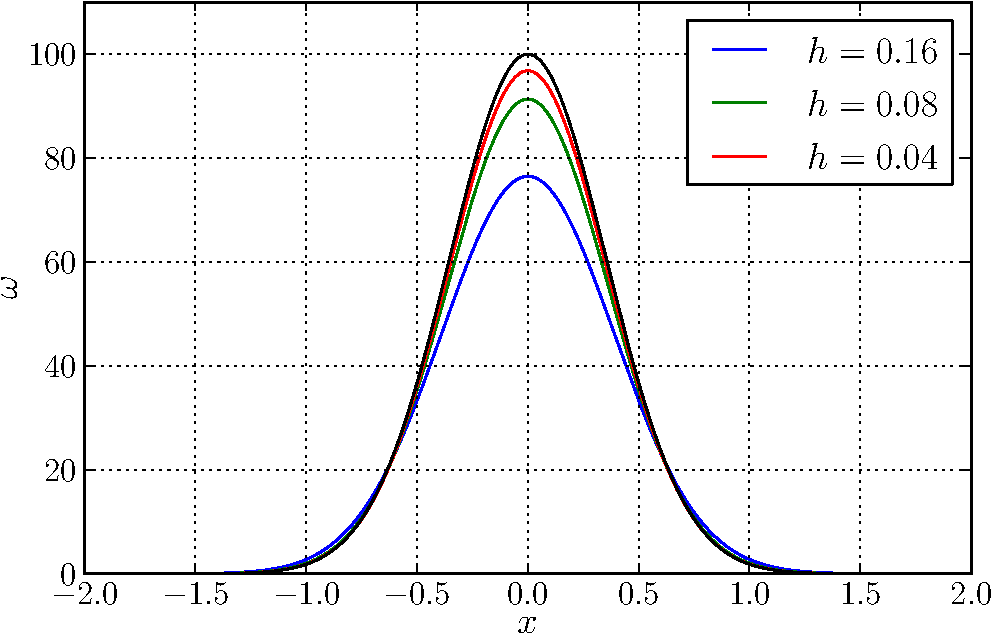
\includegraphics[width=\textwidth]{figures/lagrangian/betterInitialization_h-crop.pdf}
                \caption{Convergence of $h$ with $\mathrm{overlap} = 1.0$}
                \label{fig:convergenceOfBlobsH}
        \end{subfigure}%
        ~ %add desired spacing between images, e. g. ~, \quad, \qquad etc.
          %(or a blank line to force the subfigure onto a new line)
        \begin{subfigure}[b]{0.5\textwidth}
                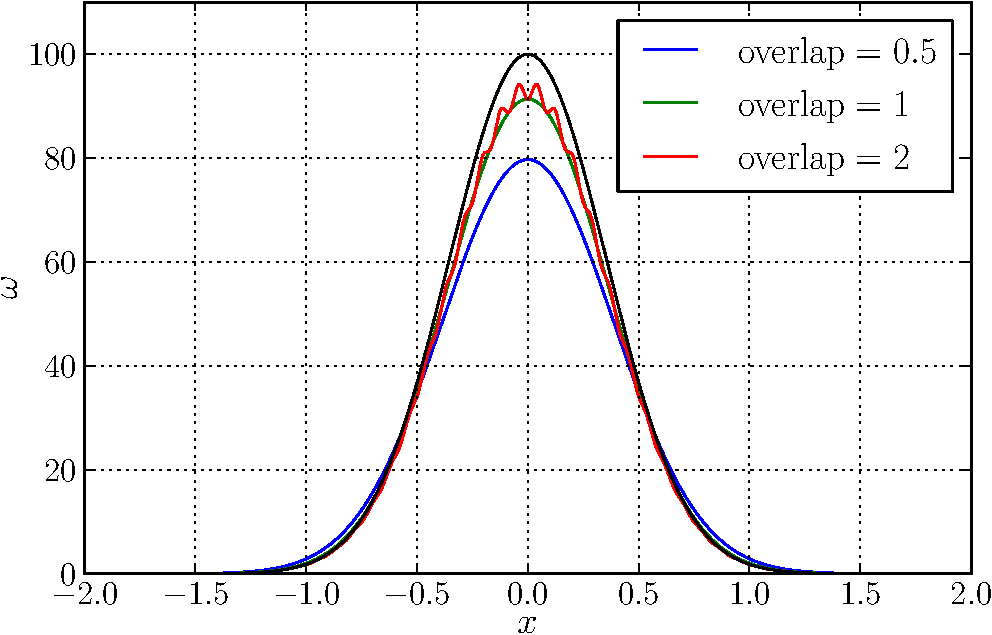
\includegraphics[width=\textwidth]{figures/lagrangian/betterInitialization_overlap-crop.pdf}
                \caption{Convergence of $\mathrm{overlap}$ with $h = 0.08$}
                \label{fig:convergenceOfBlobsOverlap}
        \end{subfigure}
        \caption{Convergence of the vorticity initialization by modifying the spatial resolution. Figure depicts exact vorticity field $\omega$ [---, solid black], the initialized vorticity distribution with various parameters.}
        \label{fig:convergenceOfSpatialResolution}
\end{figure}	

Figure \ref{fig:convergenceOfSpatialResolution} shows mollified vorticity field results from modifying the spatial resolution parameters. Figure \ref{fig:convergenceOfBlobsH} shows the convergence of the mollified vorticity field $\omega^h$ to the exact vorticity field $\omega$ by reducing the nominal particle spacing $h$. The overlap ratio is set to $\mathrm{overlap} = 1$, meaning that the blob core-size $\sigma$ is equal to $h$. We see that by reducing blob core size, and simultaneously increasing the number of particles, the mollified vorticity converges to the exact vorticity. 

The second parameter we can adjust is the $\mathrm{overlap}$ of the blobs, as seen in figure \ref{fig:convergenceOfBlobsOverlap}. The blob spacing $h$ is set to $h = 0.08$, and we see that by increasing the overlap number, the mollified vorticity approaches the exact vorticity field. However, as shown by Koumoutsakos \cite{Cottet2000a}, if the overlap is too low, we lose the smooth recovery of the vorticity field. This can be seen when the $\mathrm{overlap} = 2.0$. We see that the mollified vorticity field has a fluctuating solution. This would results in non-smooth velocity field which is an acceptable solution.

Therefore, to minimize the error between the mollified vorticity field and the exact vorticity field, we will use an $\mathrm{overlap} = 1.0$, and reduce the nominal blob spacing $h$ to a minimum. The advantage of this approach is that we can employ this correcting in a finite domain unlike the Beale's correction. However, as this correction method only minimizes the effect and not directly solve the problem of mismatched vorticity fields, it is recommended that we find a solution to this problem in future.

\section{Convection of vortex blobs}

The convection equation \ref{eq:convectionEulerian} of the viscous-splitting algorithm, is solved as system of ODEs, where,
	\begin{equation}
	\frac{\mathrm{d}\mathbf{x}_p}{\mathrm{d}t} = \mathbf{u}\left(\mathbf{x}_p\right),
	\label{eq:convectionODE}
	\end{equation}
with
	\begin{equation}
	\frac{\mathrm{d}\alpha_p}{\mathrm{d}t} = 0.
	\label{eq:conservationODE}
	\end{equation}

This problem in now solved using a Lagrangian formulation where the vortex blobs is used to discretize the vorticity field. Using the Biot-Savart law, equation \ref{eq:discreteVelocity}, we can determine the induced velocities acting on each particles. The calculation of the induced velocities an $N$-body problem and is parallelized using GPU hardware and simplified using an FMM approach.

Once we determine the induced velocity acting on each vortex blobs, they can be convected using the equation \ref{eq:convectionODE}. To retain accuracy during the convection process, we used a $4^{\mathrm{th}}$ order Runge-Kutta method, an explicit time marching scheme. As the diffusion is done at the next sub-step, the strengths of the particles do not change during the convection process.

\subsection{Remeshing scheme: Treating lagrangian grid distortion}
\label{subsec:remeshing}

	\begin{figure}[t]
	\centering
	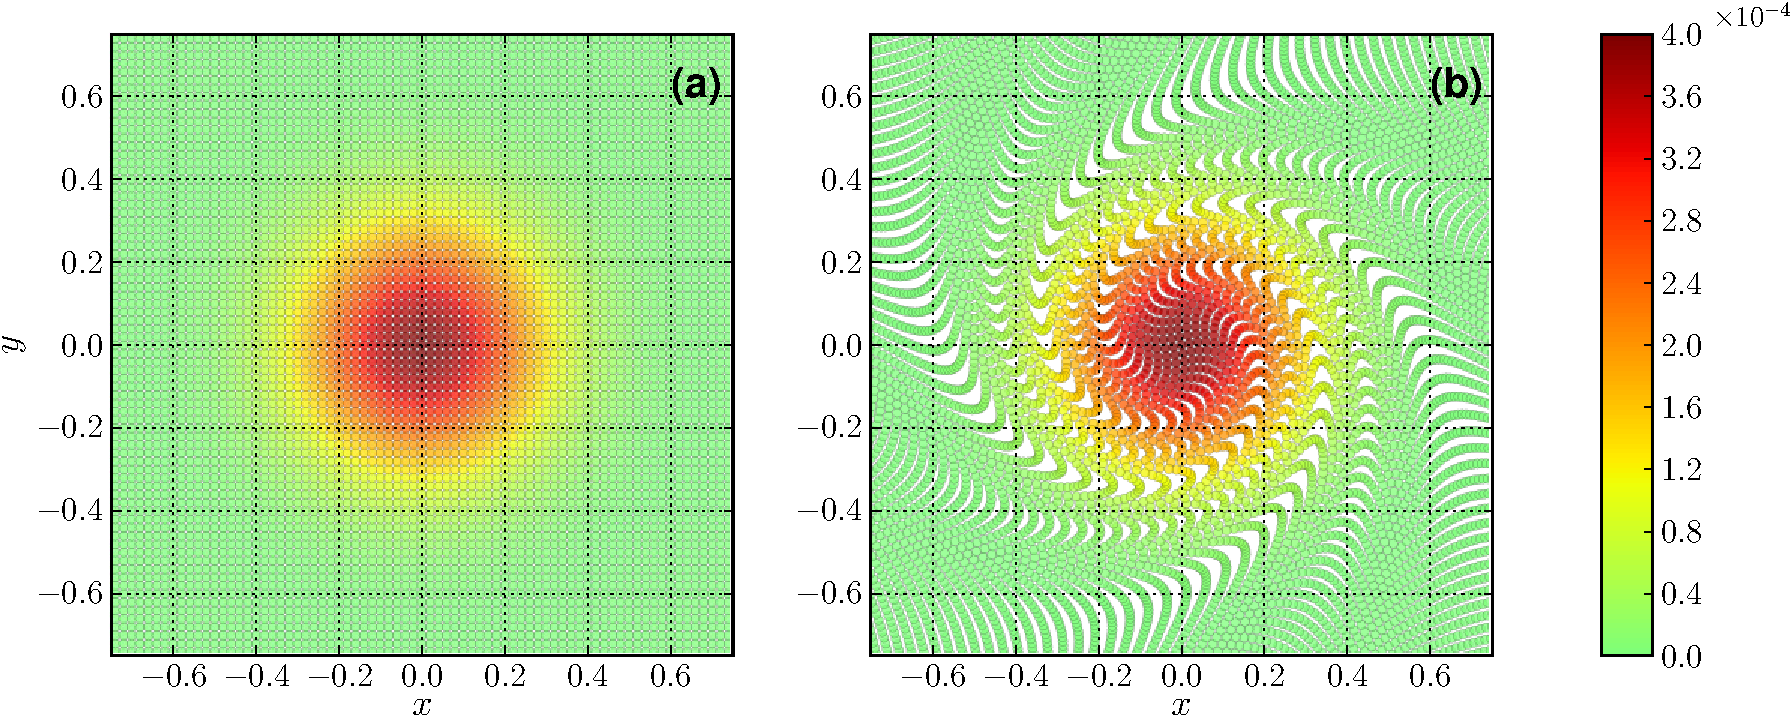
\includegraphics[width=0.9\textwidth]{figures/lagrangian/distortion-crop.pdf}
    \caption{Lagrangian distortion of the vortex blobs after 100 time steps. The initial vorticity field is $\omega\left(\mathbf{x},0\right) = \exp\left(-12\left|\mathbf{x}\right|\right)$ with $\Delta t = 0.1$, $\sigma=0.02$, and $\mathrm{overlap} = 1.0$. Figure depicts $\textbf{(a)}$ the initial distribution of the vortex blobs, and $\textbf{(b)}$ the final distribution of the vortex blobs after 100 time steps.}
    \label{fig:distortion}
	\end{figure}

During the convection step, the vortex blobs will start to cluster together at certain regions of the flow, where as at the other regions, we see that there are no blobs. This clustering and dispersing effect of the blobs is due to the high strains in the flow, figure \ref{fig:distortion}. This means that the overlap ratio is not satisfied everywhere in the flow. As we have seen before, in figure \ref{fig:convergenceOfBlobsOverlap}, overlap ratio has a large impact on the mollified vorticity field and must be satisfied. In order to treat this Lagrangian grid distortion, we can remesh the vortex blobs on to a uniform grid, regaining our intended overlap ratio.

The remeshing is done by interpolating the strengths of the vortex blobs from distorted lagrangian grid on to a uniform grid. The strengths of the blobs of the new uniform grid is defined as,
	\begin{equation}
	\alpha_p = \sum_q\tilde{\alpha}_q W \left(\frac{x_p - \tilde{x}_q}{h}\right),
	\end{equation}
where the strengths of the blobs $\tilde{\alpha}_q$ of the distorted Lagrangian grid $\tilde{x}_q$ is transfered to the regular Lagrangian grid $x_p$ using the interpolation kernel $W$. Figure \ref{fig:interpolationGrid} shows the remeshing of one vortex blob of the distorted grid on to the structured uniform grid. During this transfer, we must ensure that the properties of the fluid are conserved. The interpolation kernel is constructed by ensuring that the circulation, the linear impulse, and the angular impulse of the fluid is conserved. For this project, we used the $\mathrm{M}'_4$ interpolation kernel.

	\begin{figure}[t]
	\centering
	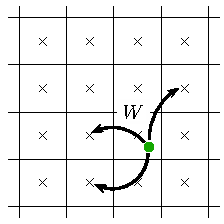
\includegraphics[width=0.4\textwidth]{figures/lagrangian/interpolationGrid.pdf}
	\caption{Remeshing of a single vortex blob [{\color{plotGreen}{$\bullet$}}, green dot] onto a uniform grid defined by the $\left(4\times4\right)$ 2-D stencil.}
	\label{fig:interpolationGrid}
	\end{figure}

\subsubsection*{$\mathbf{M}^\prime_4$ interpolation kernel}

The $\mathrm{M}^{\prime}_4$ interpolation kernel is an efficient interpolation kernel that has been used to reconstruct a smooth distribution, and was introduced by Monaghan in 1985 \cite{Monaghan1985}. For a \indexAcron{One-Dimensional}{1-D} problem, the $\mathrm{M}'_4$ interpolation kernel is given as,
	\begin{equation}
	{\mathrm{M'}_4}\left( {\xi} \right) =
	  \begin{cases}
	   {1 - \frac{{5{\xi ^2}}}{2} + \frac{{3{{\left| \xi  \right|}^3}}}{2}} & {\left| \xi \right|} < 1, \\
	   \frac{1}{2}{\left( {2 - \left| \xi  \right|} \right)^2}\left( {1 - \left| \xi  \right|} \right) & 1 \leqslant {\left| \xi \right|} < 2,\\
	   0 & 2 \leqslant \left| \xi \right|,
	  \end{cases}
	\label{eq:interpKernel}
	\end{equation}
where
	\begin{equation}
	\xi = \frac{x_{\nu} - x_i}{h},
	\label{eq:xiEquation}
	\end{equation}
	
is a non-dimensional parameter, relating the position of the particle $x_{\nu}$ to the position of the $i^{\mathrm{th}}$ interpolation node $x_i$. The $\mathrm{M'}_4$ is a third-order accurate, piecewise smooth, B-spline kernel, and with the $m = 4$, it has 4 support nodes in each dimension. Figure \ref{fig:interpolationKernel} shows the distribution of the kernel. For the two dimensional problem, the 2-D interpolation kernel is just the tensor product of the 1-D interpolation kernel, and will have a $4^2 = 16$ support nodes, as seen in figure \ref{fig:interpolationGrid}.

	\begin{figure}[t]
	\centering
	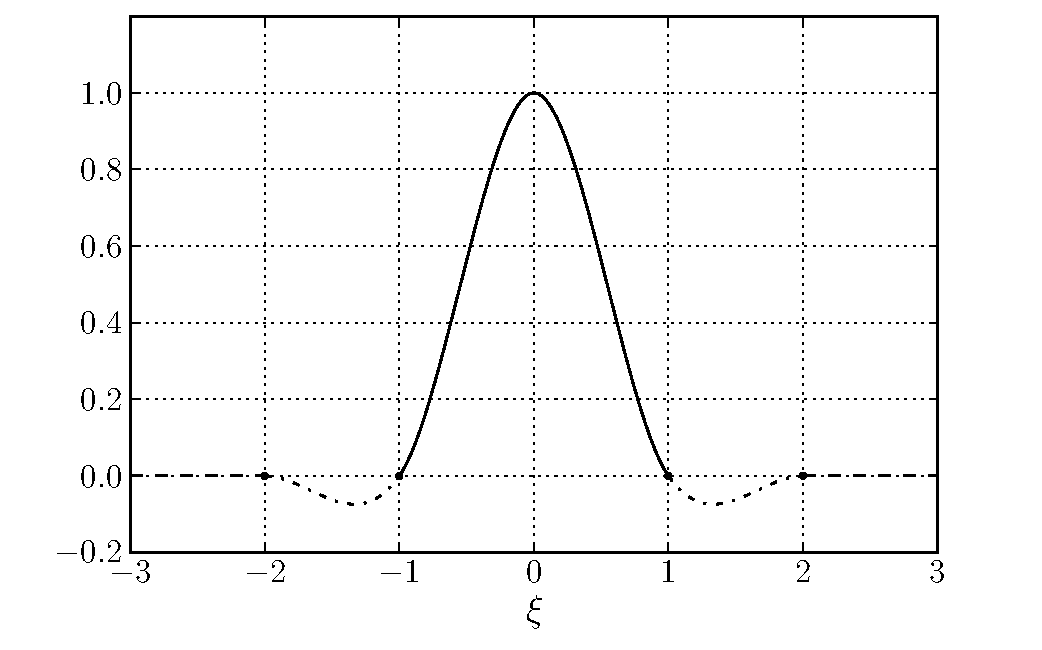
\includegraphics[width=0.7\textwidth]{figures/lagrangian/interpolationKernel.pdf}
	\caption{$M'_4$ interpolation kernel, a third-order, piecewise smooth, B-spline kernel by Monaghan \cite{Monaghan1985}}
	\label{fig:interpolationKernel}
	\end{figure}

%Koumoutsakos \cite{Koumoutsakos1997} has investigated the drawback of the employing the remeshing strategy and have shown that there is approximately $4\%$ decay in enstrophy of the flow due to sub-grid dissipation. Note that enstrophy $ \mathcal{E}$, is defined as
%
%% 4 % , give context, what time, how many remshings, say they are negligible for what we do.
%
%	\begin{equation}
%	\mathcal{E} = \frac{1}{2}\int_S \omega^2 dS
%	\end{equation}
%	
%and is directly related to the kinetic energy of the fluid and gives and insight in the energy production and the dissipation of the fluid. Enstrophy is especially useful in turbulence flow investigation as it helps describe the energy cascade of the fluid.		

\section{Diffusion of Vortex Methods}
\label{sec:diffusionVM}

So far, we have ignored the viscous effect of the flow, and in order to simulate a real flow, we must perform the diffusion of the vorticity field. Chorin simulated a viscous flow using the viscous splitting algorithm. The flow is segregated to inviscid and viscous component and during the second sub-step we deal with the diffusion of the vorticity, as show in equation \ref{eq:vsa2}. The diffusion term of the viscous splitting algorithm can be solved as a system of ODEs, similar to the convection step, given as,
	\begin{equation}
	\frac{\mathrm{d}\mathbf{x}_p}{\mathrm{d}t} = 0,
	\end{equation}
with
	\begin{equation}
	\frac{\mathrm{d}\alpha_p}{\mathrm{d}t} = \nu\Delta\alpha_p.
	\end{equation}

So in the diffusion step, we fix the position of the vortex blobs, and only modify the strengths of the particles. This process mimics the diffusion of vorticity. Chorin in 1973 \cite{Chorin1973a}, initially employed the \indexAcron{Random Walk Method}{RWM}, which generates and disperse vorticity using pseudo-random number algorithm. However, this method suffers some limitations in accuracy, and since then methods such as \indexAcron{Particle Strength Exchange}{PSE} method \cite{Degond1989a}, has been a common approach to treat the diffusion.

\subsubsection*{Particle Strength Exchange}
The Particle Strength Exchange method, first proposed by Mas-Gallic in 1989 \cite{Degond1989a}, showed that diffusion can be treated for a particle method with an isotropic, or an anisotropic viscosity by approximating the diffusion operator (a Laplacian) with an integral operator, and discretize the method with particles \cite{Speck2011a}. %The PSE can be seen as circulation correction method, where during the diffusion step of the viscous splitting algorithm, the strengths of the particle are corrected such that it accounts for the diffusion.
 
\subsubsection*{Vortex Redistribution Method}
An alternative method to simulate the diffusion is to use the \printAcron{Vortex Redistribution Method}{VRM} \cite{Shankar1996}. The model simulates diffusion by distributing the fraction of circulation of the vortex blobs to each other satisfying the diffusion. The model is based on conserving the moments of the particles by satisfying a linear system of equations. The circulation of the particle are transfer to the nearby particles that are,
	\begin{equation}
	h_{\nu} = \sqrt{\nu\Delta t_d}
	\end{equation}
where $h_{\nu}$ is the diffusion distance and is directly related to the kinematic viscosity $\nu$ and the diffusive time-step $\Delta t_d$ of the simulation. This means that the VRM scheme (and also the PSE) requires a search algorithm to determine the particles that are within the zone of influence. A direct evaluation would require an $\mathcal{O}\left(N^2\right)$ evaluation. However, this can be optimized using a search tree algorithm, speeding up the search to an $\mathcal{O}\left(\log N\right)$.

%Not that the diffusive time-step $\Delta t_d$ is equal to the convective time-step $\Delta t_c$ if the diffusion process is done during every time-step. However, we can easily adjust the diffusion time-step and perform diffusion at a multiple step of the convection. Not diffusing at every step can be helpful as 

%The downside of the this approach, as also for the standard remeshing approach is the global remeshing generates large computation data and scales with the number of particles $N$. Therefore for problems with large number of particles, a tree-structured remeshing would be more feasible strategy \cite{Winckelmans1996}.

\subsection{Modified remeshing for treating diffusion}
\label{subsec:modifiedRemeshing}
From further investigation of the VRM, Ghoniem and Wee saw that the VRM is similar to the remeshing strategy that we used to counter the lagrangian distortion during the convection process. So, Ghoniem and Wee in 2006 \cite{Wee2006a}, proposed to combine the remeshing and the diffusion together in one process. The application of this methodology was later validated by Speck in 2011 \cite{Speck2011a}. This \indexAcron{Modified Remeshing Scheme}{MRS}, performs diffusion by modifying the interpolation kernel of the remeshing scheme. The key advantage of the MRM is that, now we are dealing with a uniform grid, and no longer requires a search algorithm to find the particles in the zone of influence. This significantly reduced the computational cost, making this diffusion scheme practical for a large scale simulations. 

Ghoniem and Wee rederived the interpolation kernel that can perform both the remeshing and the diffusion simultaneously. The kernel transfers the correct fraction of circulation during the remeshing such that it satisfies the diffusion equation. The $\mathrm{M'}_4$ kernel for treating the diffusion is given as,
	\begin{equation}
	{{{\rm{M'}}}_4}\left( {\xi ,c} \right) =
	  \begin{cases}
	   {1 - \frac{{5{\xi ^2}}}{2} + \frac{{3{{\left| \xi  \right|}^3}}}{2} - {c^2}\left( {2 - 9{\xi ^2} + 6{{\left| \xi  \right|}^3}} \right)} & {\left| \xi \right|} < 1, \\
	   \frac{1}{2}{\left( {2 - \left| \xi  \right|} \right)^2}\left( {1 - \left| \xi  \right|} \right) - {c^2}{\left( {2 - \left| \xi  \right|} \right)^2}\left( {1 - 2\left| \xi  \right|} \right) & 1 \leqslant {\left| \xi \right|} < 2,\\
	   0 & 2 \leqslant \left| \xi \right|,
	  \end{cases}
	\label{eq:modInterpKernel}
	\end{equation}
where 
	\begin{equation}
	c^2 = \frac{\nu \Delta t_d}{h^2},
	\label{eq:c2}
	\end{equation}
is a non-dimensional number that corresponds to the transfer weight for the diffusion. This additional terms in the interpolation kernel accounts for the diffusion process. When $c \rightarrow 0$, the interpolation kernel simply turns in to the standard remeshing kernel. Ghoniem and Wee also investigated the error growth and the stability properties of the interpolation kernel in the Fourier space and have determined that for a stable diffusion and remeshing, we have to ensure that,
	\begin{equation}
	\frac{1}{6} \leqslant c^2 \leqslant \frac{1}{2}.
	\label{eq:c2stability}
	\end{equation}

%to minimize the error growth amplification factor and the phase error. With this, we will ensure the stability of the problem and suppress any spurious oscillations and ensure that it is a non-negative interpolation kernel with non-negative redistribution fractions. 
However, we see that this $c^2$ constraint imposes a direct constraint on the maximum and the minimum $\Delta t_d$. This would mean that the diffusion time step size $\Delta t_d$ will be a multiple of the convection step $\Delta t_c$,
	\begin{equation}
	\Delta t_d = k_d \cdot \Delta t_c,
	\end{equation}
so the diffusion of the vortex blobs will not be done at every step of the evolution process. This is a problem for hybrid method as we couple the Lagrangian and the Eulerian method at every step. If the Lagrangian method does not perform diffusion at every step, from the Eulerian method's point of view, it would seem that the Lagrangian vorticity diffuses in a discontinuous fashion. This discontinuous behavior of the Lagrangian method (w.r.t. the Eulerian method), can cause stability issues during the coupling process, and should take care of.

We could minimize this problem by modifying the $\Delta t_c$ such that it matches the diffusion time step (i.e $\Delta t_c = \Delta t_d$), so the diffusion is performed at every step. This was a feasible solution for our initial investigations with low Reynolds number flows, however when had to deal with the high Reynolds number flows, where the convection time step have to be small, we needed a scheme that was not constrained by the minimum diffusion time step.

\subsubsection*{Simple redistribution scheme}
\label{subsubsec:srs}
The simple redistribution scheme, based on the Shankar and Van Dommelen \cite{Shankar1996}, developed by Tutty in 2010 \cite{Tutty2010a}, makes it possible to remesh and diffuse the vorticity after every convection step. The strengths of the particles after the remeshing and diffusion is given as, 
	\begin{equation}
	\alpha_i^{n+1} = \sum_k \alpha_k^n W_{ki}^n, 
	\end{equation}
where $W_{ki}^n$ is the fraction of circulation from vortex blob $k$ transferred to vortex blob $i$ by the redistribution during the time step $n$. Like the MRS for treating diffusion, section \ref{subsec:modifiedRemeshing}, this \indexAcron{Simple Redistribution Scheme}{SRS} works by transferring the strengths of the particles to a fixed nodes rather than the neighboring nodes, figure \ref{fig:simpleRedistribution}. Therefore, if we use a uniform nodes, we do not need to employ a search algorithm to determine the neighboring nodes of the interpolation kernel. This makes the scheme as efficient as the MRS.

The fractions $W_{ki}^n$ are calculated by conserving the vorticity, the center of the vorticity, the linear, and the angular momentum of the vortex blobs \cite{Tutty2010a}. For the two dimensional problem, the redistribution fractions are simple tensors products of the $x,y$ one dimensional redistribution fractions, given as,

	\begin{figure}[t]
	\centering
	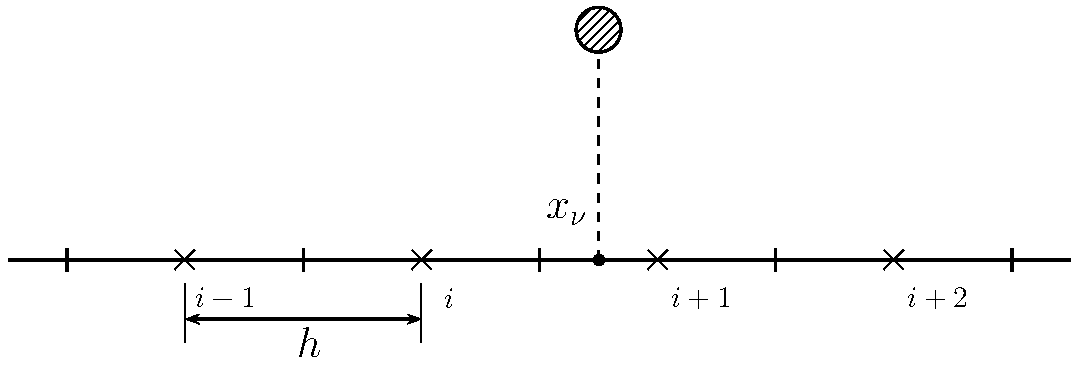
\includegraphics[width=0.7\textwidth]{figures/lagrangian/simpleRedistribution.pdf}
	\caption{One dimensional simple redistribution scheme, diffusing the vortex blobs at $x_i \leqslant x_{\nu} \leqslant x_{i+1}$, onto the four stencil points $k=i-1,\dots,i+2$, with a grid spacing $h$.}
	\label{fig:simpleRedistribution}
	\end{figure}

	\begin{equation}
	W_{kl} = F_k G_l, \quad k = i-1,\cdots,i+2, \quad \l = j-1,\dots,j+2,
	\end{equation}
giving it a 16 point stencil. The one-dimension redistribution fractions for $x$-direction is a linear combination of the two basis solution for a conservative redistribution,
	\begin{equation}
	F_k = \left(1-\Delta\right)\cdot f_k + \Delta\cdot g_k, \quad k = i-1,\dots,i+2,
	\end{equation}
having a four point stencil, as show in figure \ref{fig:simpleRedistribution}. The basis solution of redistribution are 
	\begin{subequations}
	\begin{align}
	f_{i-1} &= \frac{1}{2}\left(1-f_i-\xi\right)\\
	f_i &= 1 - 2\left(\frac{h_{\nu}}{h}\right)^2 - \xi^2\\
	f_{i+1} &= \frac{1}{2}\left(1-f_i+\xi\right)\\
	f_{i+2} &= 0
	\end{align}
	\end{subequations}
and 	
	\begin{subequations}
	\begin{align}
	g_{i-1} &= 0\\
	g_{i} &= \frac{1}{2}\left(1-g_{i+1}-\xi_1\right)\\
	g_{i+1} &= 1 - 2\left(\frac{h_{\nu}}{h}\right)^2 - \xi_1^2\\
	g_{i+2} &= \frac{1}{2}\left(1-g_{i+1}+\xi_1\right)
	\end{align}
	\end{subequations}
where $\xi$ is given by equation \ref{eq:xiEquation}. The $\xi_1 = \xi - 1$ is the distance between the $k^{\mathrm{th}}$ stencil node $x_k$ and the vortex blob that is to be diffused with $x_i \leqslant x_{\nu} \leqslant x_{i+1}$. In the above equation, $h_{\nu}$ is the characteristic diffusion distance during the time $\Delta t_d$, 
%We have to note that, $f_k$ and $g_k$ is zero for all the other $k$. 
	\begin{equation}
	h_{\nu} = \sqrt{\Delta t_d \cdot \nu}.
	\end{equation}
		
The only constraint imposed for a positive redistribution fraction is,
	\begin{equation}
	\frac{h_{\nu}}{h} < \frac{1}{\sqrt{2}}.
	\end{equation}
giving us the maximum time step size constraint of,
	\begin{equation}
	\Delta t_d < \frac{h^2}{2\nu}.
	\end{equation}
	
So we see that, this scheme only posses a constraint on the maximum diffusion time step size. For high Reynolds number flows, the convection time step is usually much smaller than the diffusion time step, meaning that now we can ensure that diffusion is performed with every convection step (i.e $k_d = 1$).

\section{Boundary conditions at solid boundary}
\label{sec:boundaryConditions}

So far, we have only dealt with unbounded flow. During bounded flow simulation, we must impose an addition constraint for the boundary, to simulate the flow with a geometry. Using the Helmholtz decomposition, we can have decompose the velocity field in to the rotational and the irrotational components, equation \ref{eq:helmholtz}. We can use the potential component to prescribe the boundary conditions at the solid wall boundary,
	\begin{equation}
	\mathbf{u}_{\phi} = \nabla\Phi.
	\end{equation}

The incompressibility constraint results in a Laplace's equation for the potential field and a unique solution is obtained by enforcing the wall boundary conditions,
	\begin{equation}
	\mathbf{u}_b\cdot\mathbf{\hat{n}} = \left(\mathbf{u}_{\omega} + \nabla\Phi\right) \cdot \mathbf{\hat{n}},
	\label{eq:potentialBC}
	\end{equation}
enforcing the no-through flow at the solid boundary wall, moving at $\mathbf{u}_b$, where $\mathbf{\hat{n}}$ is the normal vector of the solid boundary. The approach for determine the solution to the Laplace's equation is by Green's function formulation. This approach required a singularity distribution over the body resulting in the appropriate boundary condition. Doublets and/or source panels are used to attain the required potential such that equation \ref{eq:potentialBC} is satisfied.

\subsubsection{Linked boundary conditions}

However Koumoutsakos, Leonard and Pepin in 1994 \cite{Koumoutsakos1994b}, suggested to use vortex sheets to enforce the boundary conditions. This alternate approach of enforcing the solid boundary condition is by not to decompose the velocity field into potential and rotational but to consider the solid boundary as an extension of the vorticity field through vortex sheets $\gamma$, figure \ref{fig:noSlipVorticityField}. Due to the non-zero tangential velocity at the surface, a sudden discontinuity in the velocity field can be considered as vortex sheet. So to enforce the boundary conditions of the solid wall, we must satisfy the no slip velocity at the boundary,
	\begin{equation}
	\mathbf{u}\cdot\mathbf{\hat{s}} = \mathbf{u}_b\cdot\mathbf{\hat{s}}.
	\end{equation}

Koumoutsakos \cite{Koumoutsakos1993b}, relied only on the vortex sheets to enforce the no-slip velocity. Koumoutsakos, Leonard and Pepin's paper in 1994 \cite{Koumoutsakos1994b} stated that, by satisfying no-slip boundary condition, it directly satisfies the no-through boundary conditions, as these boundary conditions are linked. This was also been stated by Shiels \cite{Shiels1998} and have been further employed by Cooper, Mar and Barba in 2009 \cite{Cooper2009a}. So enforcing the no-slip boundary condition directly satisfies the no-through constraint at the surface.

	\begin{figure}[t]
	\centering
	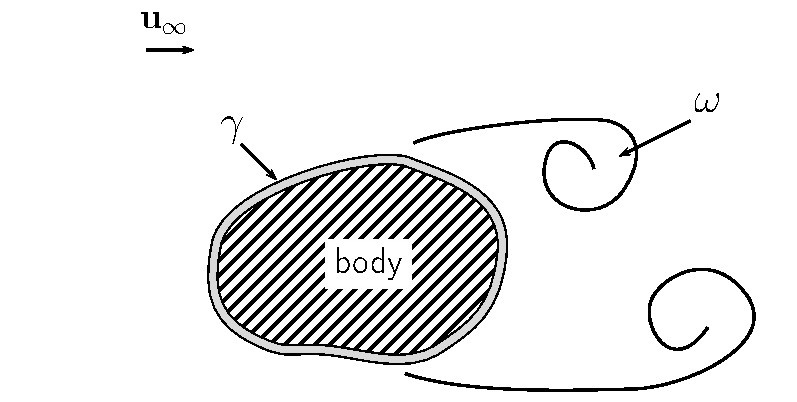
\includegraphics[width=0.6\textwidth]{figures/lagrangian/noSlipVorticityField.pdf}
	\caption{Extended vorticity field separated into vorticity in the fluid and the vortex sheet distribution confined to the body.}
	\label{fig:noSlipVorticityField}
	\end{figure}

\subsection{Boundary integral equations}

The Lagrangian method that we are using for the hybrid scheme, is modified according Stock \cite{Stock2010a}. The Lagrangian method under-resolved the vorticity field in the near-wall region. Furthermore, the vorticity of the fluid is segregated between the vortex blob domain and the vortex sheet domain, as seen in figure \ref{fig:extendedVorticityField}. The figure shows that, very near the wall the vorticity of the fluid is represented by the vortex sheet. In other words, the vortex sheet is an extension to the vorticity represented by the vortex blobs. The extended velocity field (of the extended vorticity field) is summarized as,
	\begin{equation}
	\mathbf{u} = \mathbf{u}_{\omega} + \mathbf{u}_{\gamma} + \mathbf{u}_{\infty}
	\end{equation}
where the $\mathbf{u}_{\gamma}$ denotes the velocity field induced by the vortex sheet. Enforcing the no-slip boundary conditions, we state that,
	\begin{equation}
	\left(\mathbf{u}_{\mathrm{ext}} + \mathbf{u}_{\gamma}\right)\cdot\mathbf{\hat{s}} = \mathbf{u}_b \cdot \mathbf{\hat{s}}
	\label{eq:kinematicBCofVSOutside}
	\end{equation}
where $\mathbf{u}_{\mathrm{ext}} = \mathbf{u}_{\omega} + \mathbf{u}_{\infty}$ is the velocity field induced from the vortex blob domain. The equation states that the tangential component of the total velocity acting on the body should be equal to the tangential velocity of the body. So the induced velocity of the vortex sheet is given as,
	\begin{equation}
	\left(\mathbf{u}_{\mathrm{ext}} - \mathbf{u}_b\right) \cdot \mathbf{\hat{s}} = \mathbf{u}_{\gamma}\cdot\mathbf{\hat{s}}.
	\label{eq:kinematicBCofVS}
	\end{equation}

	\begin{figure}[t]
	\centering
	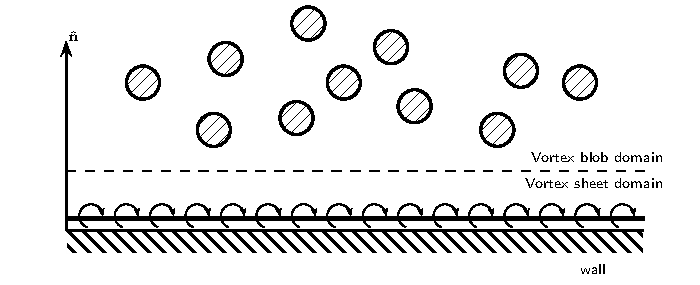
\includegraphics[width=0.8\textwidth]{figures/lagrangian/extendedVorticityField.pdf}
	\caption{Extended vorticity field: Vortex sheet being an extension to the vorticity field (resolved by the vortex blobs), capable of capturing the body bounded vorticity distribution.}
	\label{fig:extendedVorticityField}
	\end{figure}	

Note that as the boundary condition is enforced inside the body (under the vortex sheet), the velocity induced by the vortex sheet $\mathbf{u}_{\gamma}$ is the negative of equation \ref{eq:kinematicBCofVS}. Koumoutsakos \cite{Koumoutsakos1993b}, expressed the relation of the vortex sheet strengths to the no-slip boundary condition at the surface of the body (inside the body) through the Fredholm integral equation of the second kind,
	\begin{equation}
	-\frac{\gamma\left(s\right)}{2} + \frac{1}{2\pi}\oint\frac{\partial}{\partial n}\left[\log\left|\mathbf{x}\left(s\right)-\mathbf{x}\left(s'\right)\right|\right]\gamma\left(s'\right)ds'= \mathbf{u}_{\mathrm{slip}}\cdot\mathbf{\hat{s}}.
	\label{eq:fredholmIntegral2ndKind}
	\end{equation}

where $\gamma(s)$ is the strength of the vortex sheet, and $\mathbf{u}_{\mathrm{slip}} = (\mathbf{u}_{\mathrm{ext}}-\mathbf{u}_{b})$, is the slip velocity that we have to cancel. The \indexAcron{Left Hand Side}{LHS} of the equation states at the point $s$, the velocity discontinuity is due to the vortex sheet of that point and integral of all the other vortex sheets around the body. However, the equation \ref{eq:fredholmIntegral2ndKind} is not unique and accepts arbitrary solution for the vortex sheet strengths, therefore we must imposed an additional constraint on the strength of the vortex sheet. The addition constraint is a constraint on the circulation of the fluid. To ensure conservation of circulation, 
	\begin{equation}
	\Gamma = \Gamma_{\mathrm{body}} + \Gamma_{\mathrm{fluid}} = 0,
	\label{eq:circulationNet}
	\end{equation}
stating that the total circulation in the Lagrangian domain is the sum of the circulation of the body and the circulation of fluid, which should be equal to zero. As the body is in the domain of the vortex sheet, the circulation of the body is represented by the vortex sheet,
	\begin{equation}
	\Gamma_{\mathrm{body}} = \Gamma_{\gamma_{\mathrm{body}}}.
	\label{eq:circulationBody}
	\end{equation}

The circulation of the body is due to the motion of the body traveling at $\mathbf{u}_b$. One can consider the body as filled with uniform vorticity due to the rotation of the body. Therefore the circulation of a moving body can calculated simply integrating the ``vorticity'' inside the body,
	\begin{equation}
	\Gamma_b = \iint\limits_{body} \nabla \times \mathbf{u}_b \ d A.
	\end{equation}	

Furthermore, as we are using the Lagrangian method according to Stock \cite{Stock2010a}, the boundary layer of the body is not resolved with the vortex blobs, as explained in figure \ref{fig:extendedVorticityField}. Therefore, the vortex sheet has to carry this neglected circulation of the boundary layer, and the circulation of the fluid is given as,
	\begin{equation}
	\Gamma_{\mathrm{fluid}} = \Gamma_{\gamma_{\mathrm{BL}}} + \Gamma_{\omega},
	\label{eq:circulationFluid}
	\end{equation}
where $\Gamma_{\gamma_{\mathrm{BL}}}$ is the circulation of the boundary layer region represented by the vortex sheet, and $\Gamma_{\omega}$ is the total circulation captured by the vortex blobs. Combining equation \ref{eq:circulationBody} and \ref{eq:circulationFluid} into equation \ref{eq:circulationNet}, we derive the net circulation of the Lagrangian domain,
	\begin{equation}
	\Gamma = \Gamma_{\gamma_{\mathrm{body}}} + \Gamma_{\gamma_{\omega}} + \Gamma_{\omega} = 0,
	\end{equation}
where the total circulation represented by the vortex sheet is given as,
	\begin{equation}
	\Gamma_{\gamma} = \Gamma_{\gamma_{\mathrm{body}}} + \Gamma_{\gamma_{\mathrm{BL}}}.
	\end{equation}

Thus, the constraint imposed on the net circulation of the vortex sheets is given as,
	\begin{equation}
	\Gamma_{\gamma} = - \Gamma_{\omega}.
	\end{equation}	
ensuring that the total circulation of the fluid is zero. The total circulation of the vortex sheet is calculated by integrating the vortex sheet,
	\begin{equation}
	\Gamma_{\gamma} = \oint\limits_S\gamma\left(s\right)\ d s.
	\label{eq:circulationConstraintonPanels}
	\end{equation}	

So we have to solve for the vortex sheet satisfying both the equation \ref{eq:fredholmIntegral2ndKind} and the equation \ref{eq:circulationConstraintonPanels}, which can be done using a panel method.

%Now, in a pure lagrangian, we must transfer the vorticity generated from the body to the fluid. This is typically done by diffusing the vorticity of the vortex on the fluid, however in our hybrid coupling method, we can use the eulerian domain to introduce the vorticity into the fluid. The eulerian domain acts as the near-wall solver \cite{Daeninck2006}, and the strengths of the particles is interpolated from the eulerian domain, section \ref{}.\todo{CiTe Hybrid sectin}

\subsection{Panel method for treating no-slip boundary condition}
Equation \ref{eq:fredholmIntegral2ndKind} is solved by discretizing the body into $M$ vortex panels, giving us a system of $M$ equation to determine the $M$ unknowns of the strength of the vortex panels. This is the panel method, which has been extensively demonstrated by Katz and Plotkin \cite{Katz2001a}. Katz and Plotkins have shown several types of panel distributions with various orders of accuracy; from $0^{\mathrm{th}}$ order point vortex or up to $2^{\mathrm{nd}}$ order non-linear vortex panel. For this project, we have used a constant-strength vortex distribution that discretized the vortex sheet into straight segments, classified as \indexAcron{Constant-Strength Vortex Method}{CSVM}.

Panel methods are constructed by discretizing the integral equation \ref{eq:fredholmIntegral2ndKind}, and forming a system of $M$ equations to solve the $M$ unknowns of the vortex panel,
	\begin{equation}
	\underbrace{\begin{pmatrix}
	-\frac{1}{2} & a_{12} & \cdots & a_{1M}\\ 
	a_{21} & -\frac{1}{2} & \cdots & a_{2M}\\
	\vdots & \vdots & \ddots & \vdots\\ 
	a_{M1} & a_{M2} & \cdots & -\frac{1}{2}
	\end{pmatrix}}_{\mathbf{A}_{MM}} \underbrace{\begin{pmatrix}
	\gamma_{1}\\ \gamma_{2}\\
	\vdots\\
	\gamma_M\\
	\end{pmatrix}}_{\vec{\gamma}} = \underbrace{\begin{pmatrix}
	\mathrm{RHS}_1\\ 
	\mathrm{RHS}_2\\ 
	\vdots\\
	\mathrm{RHS}_M
	\end{pmatrix}}_{\overrightarrow{\mathrm{RHS}}},
	\label{eq:vortexSheetSystemofEquations}
	\end{equation}
where $A_{MM}$ contains the coefficients of the tangential induced velocity of vortex panels $\vec{\gamma}$ acting on each other. The $\overrightarrow{\mathrm{RHS}}$ is given as,
	\begin{equation}
	\mathrm{RHS} = \mathbf{u}_{\mathrm{slip}}\cdot\mathbf{\hat{s}},
	\end{equation}
and contains the boundary condition to the system of equations. In addition, we have another constraint on the net circulation of the vortex panels, equation \ref{eq:circulationConstraintonPanels}. In the discrete form, the equation is given as,
	\begin{equation}
	\sum_{i}^{M} \gamma_i\Delta s = \Gamma_{\gamma},
	\end{equation}	
and results in a $M+1$ system of equations for solving the $M$ unknown strengths of the vortex panels,
	\begin{equation}
	\underbrace{\begin{pmatrix}
	-\frac{1}{2} & a_{12} & \cdots & a_{1M}\\ 
	a_{21} & -\frac{1}{2} & \cdots & a_{2M}\\
	\vdots & \vdots & \ddots & \vdots\\ 
	a_{M1} & a_{M2} & \cdots & -\frac{1}{2}\\
	\Delta s_1 & \Delta s_2 & \cdots & \Delta s_M
	\end{pmatrix}}_{\mathbf{B}_{\left(M+1\right)M}} \underbrace{\begin{pmatrix}
	\gamma_{1}\\ \gamma_{2}\\
	\vdots\\
	\gamma_M\\
	\end{pmatrix}}_{\vec{\gamma}} = \underbrace{\begin{pmatrix}
	\mathrm{RHS}_1\\ 
	\mathrm{RHS}_2\\ 
	\vdots\\
	\mathrm{RHS}_M\\
	\Gamma_{\gamma}
	\end{pmatrix}}_{\overrightarrow{\mathrm{RHS}}},
	\end{equation}
the last equation imposing the circulation constraint on the panels. However, now we see that we have a set of $M+1$ equations with $M$ unknowns, making it an overdetermined problem. The approach to solve such a problem is either by using a \indexAcron{Least-Square solution method}{LSTSQ}, introducing a new unknown, or as used by Katz, eliminating an equation. Enforcing the no-slip boundary condition at each panel location is a vital criteria, and therefore we used the LSTSQ method for solving the problem.

\subsubsection{Constant-Strength Vortex Method}

The Constant-Strength vortex method ({\color{darkblue}CSVM}) is based on the flat (straight) discretization of the vortex sheet, where the panel have constant vortex strength. To solve the strengths of the panel problem, we enforce the Dirichlet velocity boundary conditions at the collocation point $x_{cp}$, that is located just below the vortex sheet, shown in figure \ref{fig:vortexPanelDefinition}. The coefficient $a_{ij}$ of the influence matrix $\mathbf{A}$ is defined as,
	\begin{equation}
	a_{ij} = \mathbf{\hat{u}}_{ij} \cdot \mathbf{\hat{t}}_i,
	\end{equation}
which represents the tangential influence coefficient of $j^{\mathrm{th}}$ panel on the $i^{\textrm{th}}$ panel. The influence coefficient is determined by prescribing the strengths of the vortex panels $\hat{\gamma}_i = 1$, resulting in an induced velocity $\mathbf{\hat{u}}_{ij} = \left(\hat{u},\hat{v}\right)_{ij}$ for a unit strength panel.

	\begin{figure}[t]
        \centering
        \begin{subfigure}[b]{0.5\textwidth}
                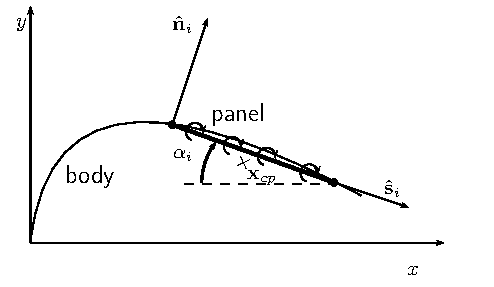
\includegraphics[width=\textwidth]{figures/lagrangian/panelCoordinateDefinition.pdf}
                \caption{Panel discretization of the body in the global cartesian coordinates system $\left(x,y\right)$ with the local panel coordinates system rotated by $\alpha_i$.}
                \label{fig:panelCoordinateDefinition}
        \end{subfigure}%
        ~ %add desired spacing between images, e. g. ~, \quad, \qquad etc.
          %(or a blank line to force the subfigure onto a new line)
        \begin{subfigure}[b]{0.5\textwidth}
                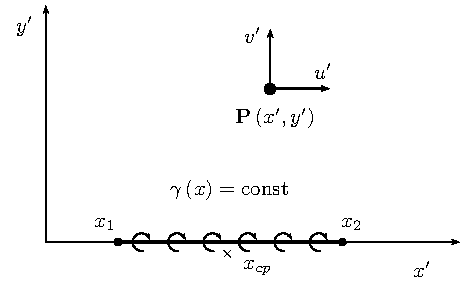
\includegraphics[width=\textwidth]{figures/lagrangian/vortexPanelDefinition.pdf}
                \caption{Constant-Strength Vortex panel in the local panel coordinate system $\left(x',y'\right)$ inducing the velocity $\mathbf{u}'=(u',v')$ on the point $P$.}
                \label{fig:vortexPanelDefinition}
        \end{subfigure}
        \caption{The two coordinate system of the panel method problem. The figure depicts \textbf{(a)} the global panel coordinate system, and \textbf{(b)} the local panel coordinates system, as defined by Katz and Plotkins \cite{Katz2001a}.}
        \label{fig:panelDefinitions}
	\end{figure}	
	
Figure \ref{fig:panelCoordinateDefinition} shows the discretization of the body into panels in the global coordinates system, defined by $(x,y)$, where each panel is rotated by an angle $\alpha_i$ w.r.t to the global coordinate system. Rotating the axis $(x,y)$ by $\alpha_i$, we arrive at the local panel coordinate system $(x',y')$, as shown in figure \ref{fig:vortexPanelDefinition}. In general, the induced velocity of the vortex panels are calculated in the local panel coordinate system, where the induced velocity of the vortex panel $j$ on the collocation point $i$ (in the panel coordinate system) is given as,
	\begin{subequations}
	\begin{align}
	u'_{ij} &= \frac{\gamma_j}{2\pi}\left[\tan^{-1}\frac{y'_i-y'_{j,2}}{x'_i-x'_{j,2}} - \tan^{-1}\frac{y'_i-y'_{j,1}}{x'_i -x'_{j,1}}\right],\\
	v'_{ij} &= -\frac{\gamma_j}{4\pi}\ln\frac{\left(x'_i-x'_{j,1}\right)^2 + \left(y'_i-y'_{j,1}\right)^2}{\left(x'_i-x'_{j,2}\right)^2+\left(y'_i-y'_{j,2}\right)^2}
	\end{align}
	\end{subequations}

where $(x'_1,y'_1)_j$ and $(x'_2,y'_2)_j$ are the coordinates of the panel start and end points in its local panel coordinate system, as shown in figure \ref{fig:panelDefinitions}. The transformation of this vector $(u'_{ij}, v'_{ij})$ to the global coordinates is given as,
	\begin{equation}
	\begin{bmatrix}
	u_{ij}\\
	v_{ij}\\
	\end{bmatrix} = \begin{bmatrix}
	\cos\alpha_j & \sin\alpha_j \\
	-\sin\alpha_j & \cos\alpha_j
	\end{bmatrix} \cdot \begin{bmatrix}
	u'_{ij}\\
	v'_{ij}.
	\end{bmatrix}
	\end{equation}

	\begin{figure}[t]
	\centering
	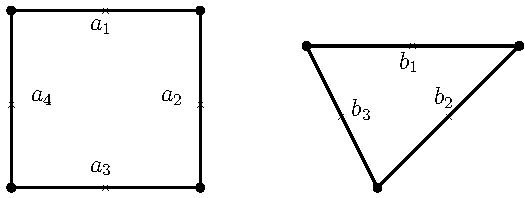
\includegraphics[width=0.6\textwidth]{figures/lagrangian/twoPanelBodies.pdf}
	\caption{Multi-body panel problem: two bodies with different numbers of panels. The figure depicts a square body with 4 panels ($a_1, a_2, a_3, a_4$), and a triangular body with 3 panels ($b_1, b_2, b_3$). }
	\label{fig:twoPanelBodies}
	\end{figure}

Note that when $i=j$, the influence coefficient becomes $a_{ij} = -1/2$, represented by the diagonal terms of equation \ref{eq:vortexSheetSystemofEquations}. If we are dealing with multiple panel bodies (i.e. multiple geometries), as seen in figure \ref{fig:twoPanelBodies}, the panel problem can be solved by constructing a global influence matrix, 
	\begin{equation}
	\underbrace{\begin{pmatrix}
		c_{a_1a_1} & \cdots & c_{a_1a_N} & c_{a_1b_1} &\cdots & c_{a_1b_M}\\
		\vdots & \ddots & \vdots & \vdots &\ddots & \vdots\\
		c_{a_Na_1} & \cdots & c_{a_Na_N} & c_{a_Nb_1} &\cdots & c_{a_Nb_M}\\
		c_{b_1a_1} & \cdots & c_{b_1a_N} & c_{b_1b_1} &\cdots & c_{b_1b_M}\\
		\vdots & \ddots & \vdots & \vdots &\ddots & \vdots\\
		c_{b_Ma_1} & \cdots & c_{b_Ma_N} & c_{b_Mb_1} &\cdots & c_{b_Mb_M}\\
		\Delta s_{a_1} & \cdots & \Delta s_{a_N} & 0 & \cdots & 0\\
		0 & \cdots & 0 & \Delta s_{b_1} & \cdots & \Delta s_{b_M}\\
	\end{pmatrix}
	\begin{pmatrix}
		\gamma_{a_1}\\
		\vdots\\
		\gamma_{a_N}\\
		\gamma_{b_1}\\
		\vdots\\
		\gamma_{b_M}\\
	\end{pmatrix}}_{\begin{pmatrix}
						C_{aa} & C_{ab} \\
						C_{ba} & C_{bb} \\
						\Delta s_a & 0\\
						0 & \Delta s_b \\
					\end{pmatrix} \begin{pmatrix}
								\gamma_{a}\\
								\gamma_{b}\\
							\end{pmatrix}} 
	= 
	\underbrace{\begin{pmatrix}
		\mathrm{RHS}_{a_1}\\
		\vdots\\
		\mathrm{RHS}_{a_N}\\
		\mathrm{RHS}_{b_1}\\
		\vdots\\
		\mathrm{RHS}_{b_M}\\
		\Gamma_{\gamma,a}\\	
	\Gamma_{\gamma,b}
	\end{pmatrix}}_{ 
			\begin{pmatrix}
				\mathrm{RHS}_{a}\\
				\mathrm{RHS}_{b}\\
				\Gamma_{\gamma,a}\\	
				\Gamma_{\gamma,b}
			\end{pmatrix}}
	\end{equation}

where the diagonal matrices ($C_{aa}$, $C_{bb}$), are the self-induction matrix of the panel body, $a \rightarrow a$ and $b \rightarrow b$ respectively. The non-diagonal terms ($C_{ab}$, $C_{ba}$) are the inter-induction matrix containing the panel influence of $b\rightarrow a$ and $a\rightarrow b$ respectively. The final two rows of the LHS matrix contains the circulation constraint for each body.

%\newpage
%\section{Simulation acceleration techniques}
%\label{sec:sat}
%%
%\subsection{Fast multi-pole Method}
%%
%\subsection{Parallel computation in GPU}
%
\section{Validation of Lagrangian method}
During the validation study, we are will not be able to validate the vorticity generation of the Lagrangian boundary. 
This is due to the nature of the hybrid method that we are using for this project. The generation of the vorticity from the boundary is defined in the Eulerian method, which is then interpolated onto the Lagrangian domain. Therefore, test cases that relies on the generation of the vorticity from the boundary cannot be used to validate our Lagrangian method.
Thus the validation study for the Lagrangian method was done separately; first ensuring no-through flow on vortex panels is properly handled; second ensuring that the vorticity of the flow is properly handled by the vortex blobs.

\subsection{Error analysis of panel method}
The validation of the panel method was done by performing a convergence study of a cylinder. The vortex panels where used to simulate a potential flow around a cylinder and the solution of the panels were compared with the analytical solutions.

	\ctable[
	    caption = {Panel study parameters},
	    label   = {tab:panelParams},
	    pos = b,
	]{lll}{}{\FL
	Parameters 				& Value 			& Description \ML
	$R$  					& 1 \si{m} 			& Radius of cylinder\\
	$\mathbf{u}_{\infty}$	& 1 \si{m.s^{-1}}	& Free-stream velocity\\
	$N_{\mathrm{panels}}$	& 100				& Number of panels\LL}	

To test the solution of the vortex panels with the analytical solution, the problem was first ran for the parameters in the table \ref{tab:panelParams}. The velocity field of the potential flow solution is shown in figure \ref{fig:panelCylinder_velocityField}. The figure shows the magnitude of the velocity, and we see that it shows the velocity field of a potential flow solution, with an infinitely thin boundary layer, stagnating to zero velocity inside the body.

	\begin{figure}[p]
	\centering
	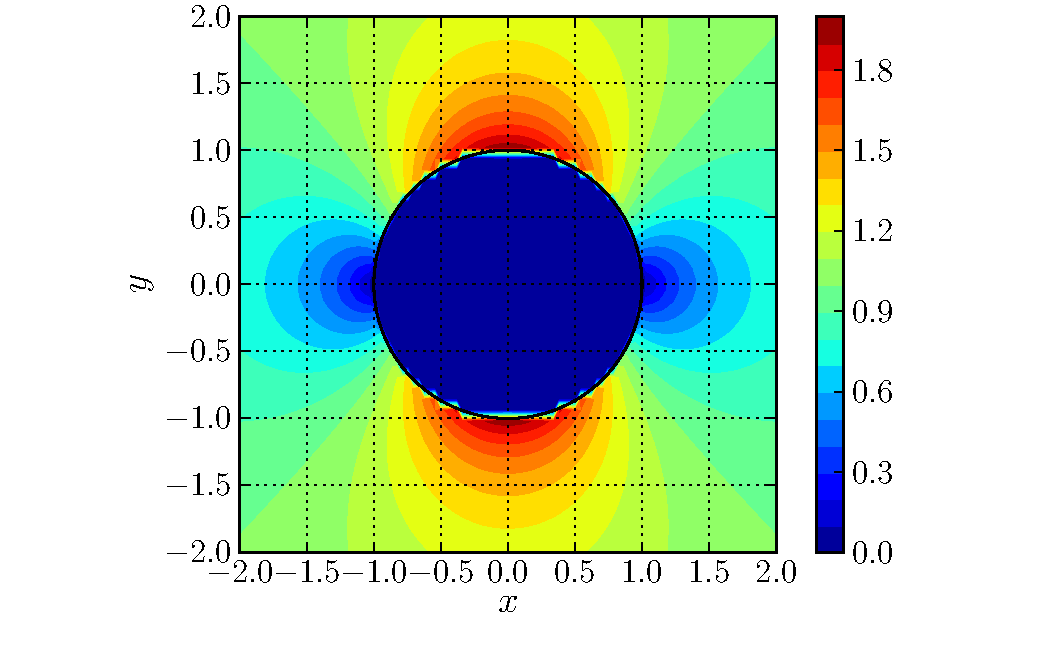
\includegraphics[width=0.7\textwidth]{figures/lagrangian/panelCylinder_velocityField.pdf}
	\caption{Panel method solution: the potential velocity field around a unit cylinder with $R = 1$, $\mathbf{u}_{\infty} = (1, 0)$, and $N_{\mathrm{panels}}=100$. The figure depicts the magnitude of velocity field $\left\Vert\mathbf{u}\right\Vert$, with a zero velocity inside the body.}
	\label{fig:panelCylinder_velocityField}
	\end{figure}

	\begin{figure}[p]
     \centering
     \begin{subfigure}[b]{0.5\textwidth}
             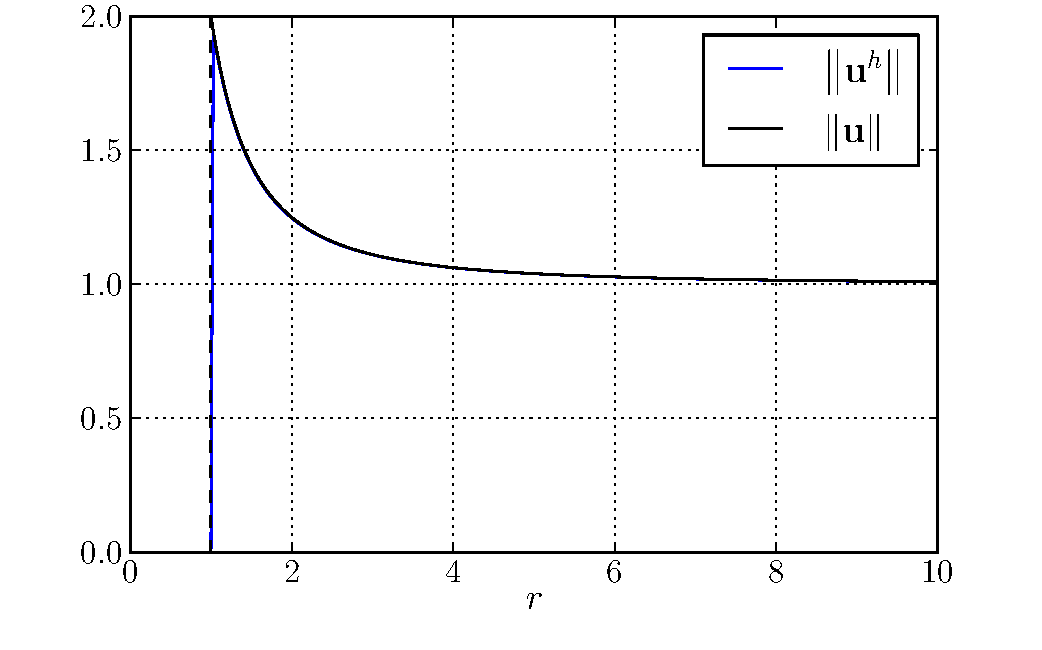
\includegraphics[width=\textwidth]{figures/lagrangian/panelCylinder_versusAnalytical.pdf}
             \caption{Comparison of the velocity field.}
             \label{fig:panelCylinder_versusAnalytical}
     \end{subfigure}%
     ~ %add desired spacing between images, e. g. ~, \quad, \qquad etc.
       %(or a blank line to force the subfigure onto a new line)
     \begin{subfigure}[b]{0.5\textwidth}
             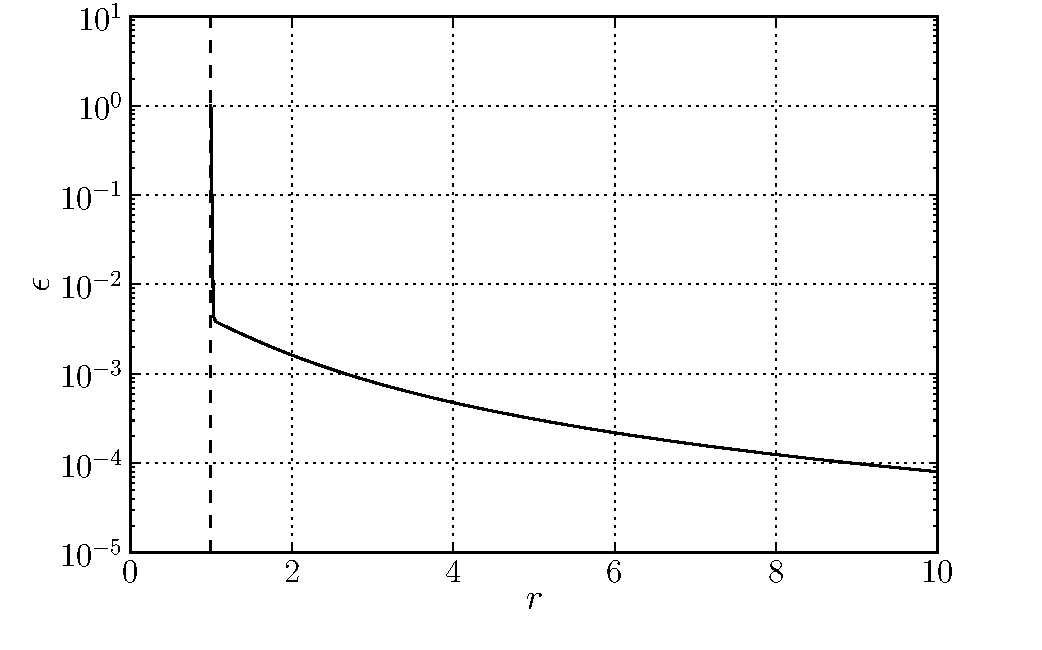
\includegraphics[width=\textwidth]{figures/lagrangian/panelCylinder_error.pdf}
             \caption{Error in the velocity field}
             \label{fig:panelCylinder_error}
     \end{subfigure}
     \caption{Comparison of the velocity field along the $y$-axis, $0\rightarrow10$. Figure \textbf{(a)} shows both the solutions, the numerical $\left\Vert\mathbf{u}^h\right\Vert$ [{\color{plotBlue}{---}}, solid blue] and the analytical solution [---, solid black]. Figure \textbf{(b)} shows the relative error $\epsilon$ in velocity between the solution, given by equation \ref{eq:panelRelativeError}.}
     \label{fig:panelCylinderComparision}
	\end{figure}

	\begin{figure}[p]
	\centering
	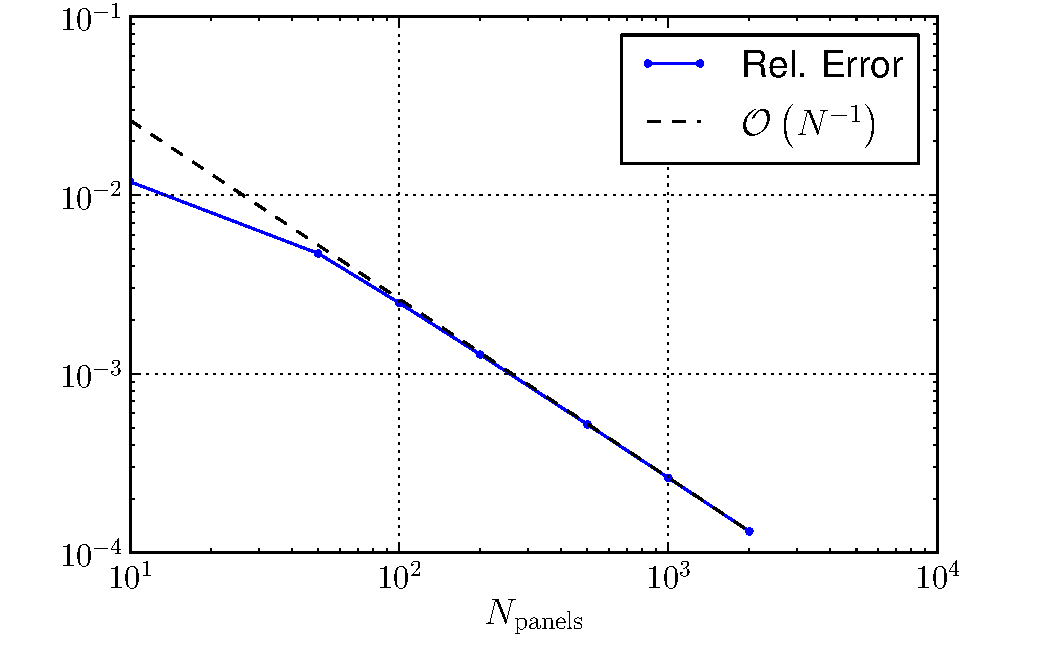
\includegraphics[width=0.5\textwidth]{figures/lagrangian/panelCylinder_convergence_compressed.pdf}
	\caption{Convergence plot of the Constant-Strength Straight Vortex panels. The figures depicts the converges of the relative error $\epsilon$ at an $\mathcal{O}\left(N^{-1}\right)$.}
	\label{fig:panelCylinder_convergence}
	\end{figure}


The jagged velocity field around the surface of the cylinder is simply due to the sampling resolution of the field, and for a higher sampling resolution, this will vanish. In order to determine the accuracy of the solution, the velocity field of the panel solution was compared with the analytical solution. The analytical velocity field around a cylinder is given as,
	\begin{subequations}
	\begin{align}
	u_r &= u\left(1 - \frac{R^2}{r^2}\right)\cos\theta,\\
	u_{\theta} &= -u\left(1+\frac{R^2}{r^2}\right)\cos\theta,
	\end{align}
	\label{eq:potentialCylinderAnalytical}
	\end{subequations}	
where $u_r$ and $u_{\theta}$ are the radial and the angular velocity respectively. The equation \ref{eq:potentialCylinderAnalytical} is a function of the radius from the center of the cylinder (in our case $r_0 = [0, 0]$) and the radius of the cylinder $R$. 

The velocity field of the vortex panel was compared with this analytical solution along the y-axis from $y=0 \rightarrow 10$. Figure \ref{fig:panelCylinder_versusAnalytical} plots the magnitude of analytical velocity $\left\Vert\mathbf{u}\right\Vert$ and the vortex panel velocity field $\left\Vert\mathbf{u}^h\right\Vert$. Comparing the solutions of the plot we see that the solution of the vortex panels and the analytical potential flow solution matches everywhere except at the surface. This happens because the potential flow solution has a slip velocity (i.e non-zero velocity) at the surface of the body, whereas the vortex panels solves for a no-slip boundary condition at the collocation points of the surface. This explains the sudden drop of the velocity from $2\rightarrow0$ at the surface.	

The figure \ref{fig:panelCylinder_error} shows the relative error $\epsilon$ between the numerical and the analytical solution,
	\begin{equation}
	\epsilon = \frac{\left\Vert\mathbf{u}-\mathbf{u}^h\right\Vert}{\left\Vert\mathbf{u}\right\Vert}
	\label{eq:panelRelativeError}
	\end{equation}
	
where $\mathbf{u}$ is the analytical solution and the $\mathbf{u}^h$ is the numerical (panel method) solution. Ignoring the solution right at the surface ($r=R$), we see that the error between the numerical and the analytical solution reduces from $\epsilon=\num{5e-3}\rightarrow \num{8e-5}$ as we go from $r=1\rightarrow10$. This behavior of the error tells us that the solution of the constant-strength vortex panels gets more accurate as we go further away from the panels; right next to the panels, we have the largest error. This is because the vortex panels discretizes the body using a first-order approximation (straight panels) and also discretizes the vortex sheet strength using a first-order approximation. 

The convergence analysis of the vortex panels was done by determine the error of the vortex panel velocity field w.r.t to the analytical solution for the number of panels $N = 10 \rightarrow 1000$, figure \ref{fig:panelCylinder_convergence}. The error of the velocity field was determine at $R = 1.5$, and we see that the error converges at an $\mathcal{O}\left(N\right)$. This validates that the vortex panel that we have used is a $1^{\mathrm{st}}$ order vortex panel.

\subsection{Evolution of the vortex blobs}

In order to verify and validate the vortex blobs, we simulate the evolution of a Lamb-Oseen vortex. The results of the simulation was used to compare against the analytical results, which we used to determine the accuracy of our vortex blobs.

\subsection*{Lamb-Oseen vortex}
\label{subsec:lagrangianLambOseen}
The Lamb-Oseen vortex is a simple solution of unbounded laminar Navier-Stokes equation of a vortex core diffusing as time passes. It was first demonstrate by Lamb and Oseen \cite{Tryggeson2007}. The vorticity distribution $\omega$ of the core at a given time is defined as,

	\begin{equation}
	\omega\left(\mathbf{x},\tau\right) = \frac{\Gamma_c}{4\pi\tau} \exp\left(-\frac{r^2}{4\tau}\right),
	\label{eq:lo_voeq}
	\end{equation}

and is a function of core strength $\Gamma_c$, the scaled viscous time $\tau$, and distance from the core center $r$. The scaled viscous time is defined as,
	\begin{equation}
	\tau \equiv \nu t.
	\end{equation}
At $\tau=0$, the Lamb-Oseen vorticity distribution is a Dirac delta function, and the core starts to diffuse and expand as the time progresses. The velocity field of the Lamb-Oseen vortex is given as,

	\begin{subequations}
	\begin{align}
	u_{\theta} &= \frac{\Gamma_c}{2\pi r} \left[1-\exp\left(-\frac{r^2}{4\tau}\right)\right]\\
	u_r &= 0
	\end{align}
	\label{eq:lo_veeq}
	\end{subequations}

where $u_{\theta}$ is the circumferential velocity, and $u_r$, the radial velocity is zero. Figure \ref{fig:lambOseen_distributions} shows the vorticity distribution, and the velocity field of the Lamb-Oseen vortex with a unit core strength $\Gamma_c=1$, at scaled viscous time $\tau=\num{2e-3}$. As the time progresses, the core of the Lamb-Oseen vortex will diffuse and we use this analytical solution to valid our vortex blobs.

	\begin{figure}[!t]
        \centering
        \begin{subfigure}[b]{0.5\textwidth}
                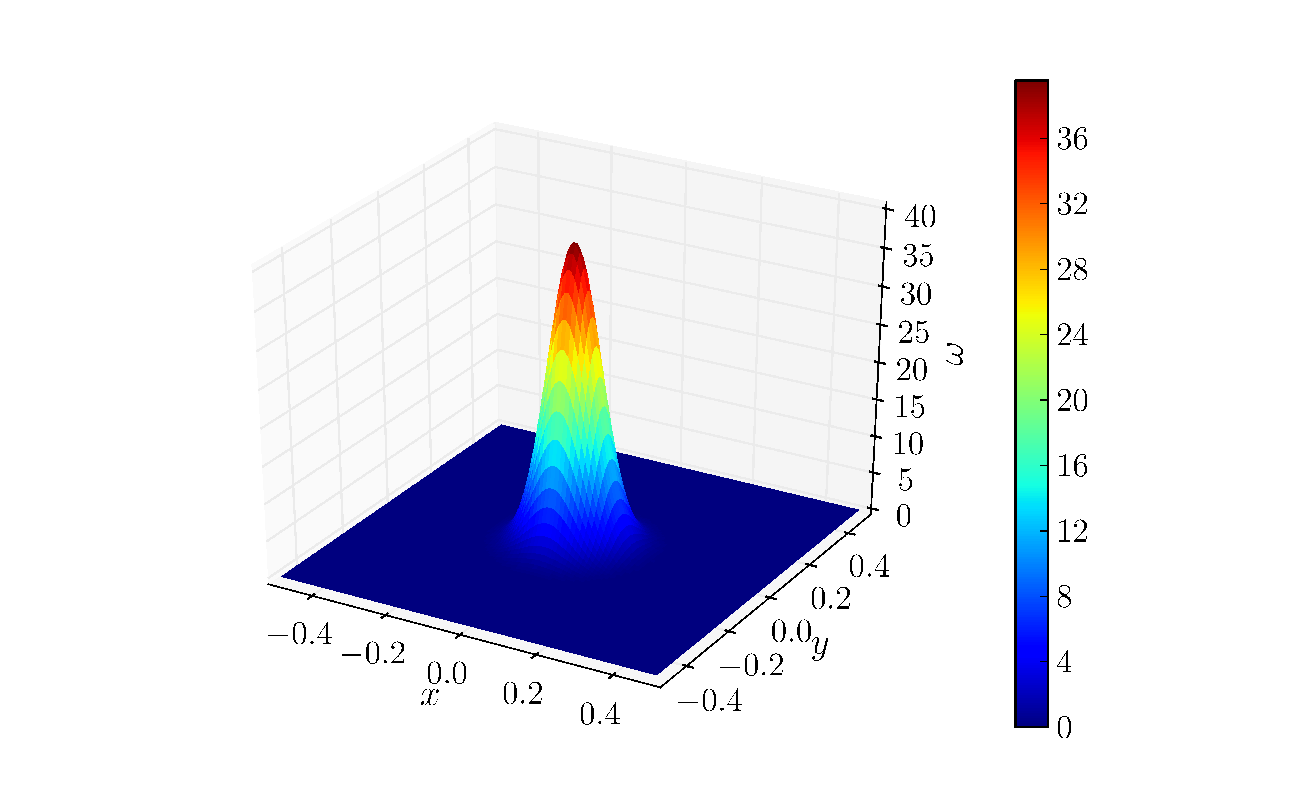
\includegraphics[width=\textwidth]{figures/lagrangian/lambOseen_vorticityDistribution_compressed.pdf}
                \caption{Vorticity field}
                \label{fig:lambOseen_vorticityDistribution}
        \end{subfigure}%
        ~ %add desired spacing between images, e. g. ~, \quad, \qquad etc.
          %(or a blank line to force the subfigure onto a new line)
        \begin{subfigure}[b]{0.5\textwidth}
                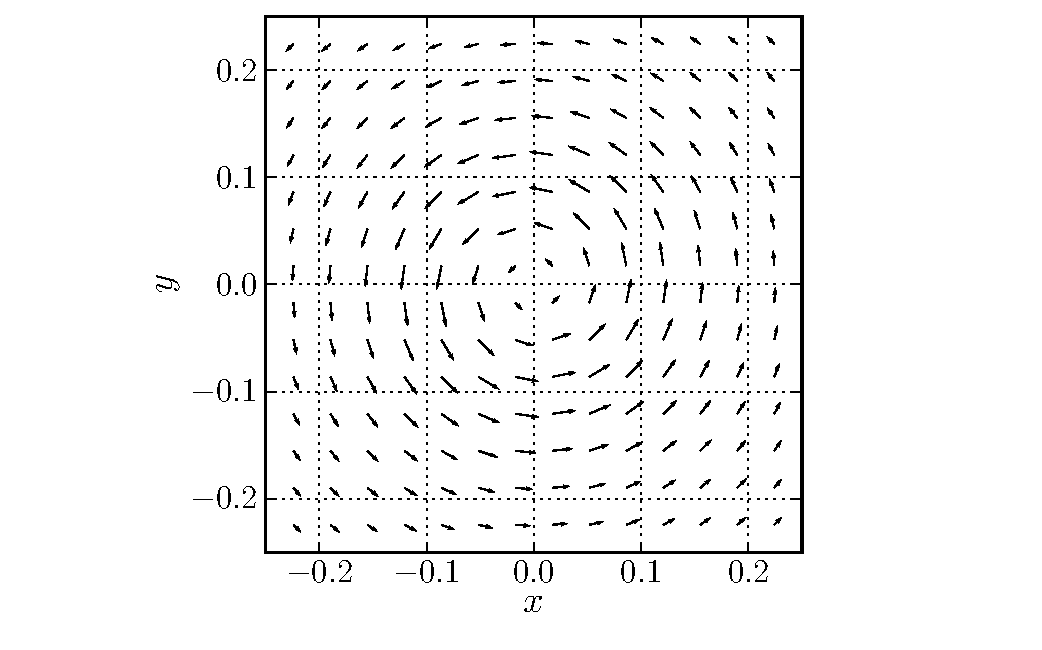
\includegraphics[width=\textwidth]{figures/lagrangian/lambOseen_velocityDistribution_compressed.pdf}
                \caption{Velocity Field}
                \label{fig:lambOseen_velocityDistribution}
        \end{subfigure}
        \caption{Lamb-Oseen Vortex problem with $\Gamma_c = 1$, $\tau=\num{2e-3}$, and $\nu=\num{5e-4}$. The figure depicts \textbf{(a)} the vorticity distribution, and \textbf{(b)} the velocity distribution.}
        \label{fig:lambOseen_distributions}
	\end{figure}

The lagrangian method ran the case of Lamb-Oseen vortex simulation according to the parameters tabulated in table \ref{tab:lambOseenParams}. The problem was initialized by discretizing the vorticity field of the Lamb-Oseen vortex with $\Gamma_c=1$, $\nu=\num{5e-4}$, and $\tau_0 = \num{2e-3}$, the initial scaled viscous time. The vorticity field was discretized over the domain $[x,y]$-domain $\left[-0.5,0.5\right]^2$ using vortex blobs with $\sigma=0.01$, and $\mathrm{overlap}=1$, giving it a fixed blob spacing of $h=0.01$. We employed the standard initialization method of vortex blobs from section \ref{subsec:vortexBlobInitialization}. 

However as explained in section \ref{subsec:vortexBlobInitialization}, we have to take in account of the gaussian blurring of the original vorticity field due to the initialization process. This posses a problem when evaluating the error between the numerical and the analytical solution. Barba \cite{Barba2004c}, had also encountered the problem before when investigating with a Lamb-Oseen vortex. The solution to the problem was to apply a ``time-shift correction", to compensate for the gaussian blurring, solving the problem of this very particular discretization of the diffusion equation. Therefore, this is a special method and this approach can only be used for the Lamb-Oseen vortex problem.

	\ctable[
		caption = {Summary of the parameters for the Lamb-Oseen vortex evolution. Table shows the parameters of Tutty's diffusion method \cite{Tutty2010a}},
		label   = {tab:lambOseenParams},
		pos = t,]{lcll}{}{\FL
		
		Parameters 					& Value 	& Unit					& Description \ML
		$\Gamma_c$\T               	& 1 &\si{m^2.s^{-1}} 				& Core strength\\
		$\Omega$               		& $\left[-0.5,0.5\right]^2$ &\si{m}	& Initial particle domain \\
		$\mathbf{u}_{\infty}$ 		& $\left[0, 0\right]$ &\si{m.s^{-1}} & Free-stream velocity\\
		$\nu$						& $\num{5e-4}$ &\si{kg.s^{-1}.m^{-1}}& Kinematic viscosity\\
		$ (\tau_0,\tau_f)$ 		    & \numrange{2e-3}{2.5e-3} &\si{m^2}	& Initial and final scaled viscous time\\
		$ (t_0,t_f)$ 		    	& \numrange{4}{5} &\si{s}			& Initial and final simulation time\\		
		$ \Delta t_c = \Delta t_d$ 	& $0.01$ &\si{s}						& Diffusion and convection time step size\\
		$ N_{\mathrm{t-steps}}$ 	& 100 & -						& Number of time integration steps\\		
		$ \sigma$ 					& $0.01$ &\si{m}						& Vortex blob core size\\	        
		$ \mathrm{overlap}$			& $1$	& -							& Overlap ratio\\	        	        
		$ k$						& $2$	& -							& Gaussian kernel width spreading\\
		$ f_{\mathrm{redist}}$		& $1$ 	& -							& Redistribution occurance\\	        	        
		$ f_{\mathrm{popControl}}$		& $1$  & -							& Population control occurance\\	        	        
		$ \Gamma_{\mathrm{threshold}}$ & $(\num{1e-14},\num{1e-14})$ &\si{m^2.s^{-1}} & Population control threshold\LL}

The ``time-shift correction" is derived by determining the diffusion effect caused by the discretization of the diffusion equation using the gaussian vortex blobs (with $k=2$). Barba determined that discretization of the diffusion equation (i.e. the Lamb-Oseen vortex) reconstructs the vorticity field that has been diffused by a time $\sigma^2/2\nu$. So when initializing the particles with a certain strength, we will have to reverse the time by $\sigma^2/2\nu$. The initial particles strengths $\alpha_0$ of vortex blobs from the Lamb-Oseen vorticity field is given as,

	\begin{equation}
	\alpha_0 = \omega_0\cdot h^2 = \left\{ \frac{\Gamma_c}{4\pi\nu\left(t-\sigma^2/2\nu\right)} \exp\left[-\frac{r^2}{4\nu\left(t-\sigma^2/2\nu\right)}\right] \right\} \cdot h^2.
	\label{eq:lo_pie}
	\end{equation}
	
This method was used to investigate the error growth of the vortex blob method. The vortex blobs where convected and diffused according to the parameters in table \ref{tab:lambOseenParams}. For the primary and the main investigation, we used diffusion method proposed by Tutty \cite{Tutty2010a}. The advantage of this approach is that the we can perform diffusion after every convection step. This makes the method less prone to time integration error and eliminates any discontinuous behaviour in the evolution. We will see that when coupling the Lagrangian method and Eulerian method, discontinuity in the problem introduces additional errors.

	\begin{figure}[p]
	\centering
	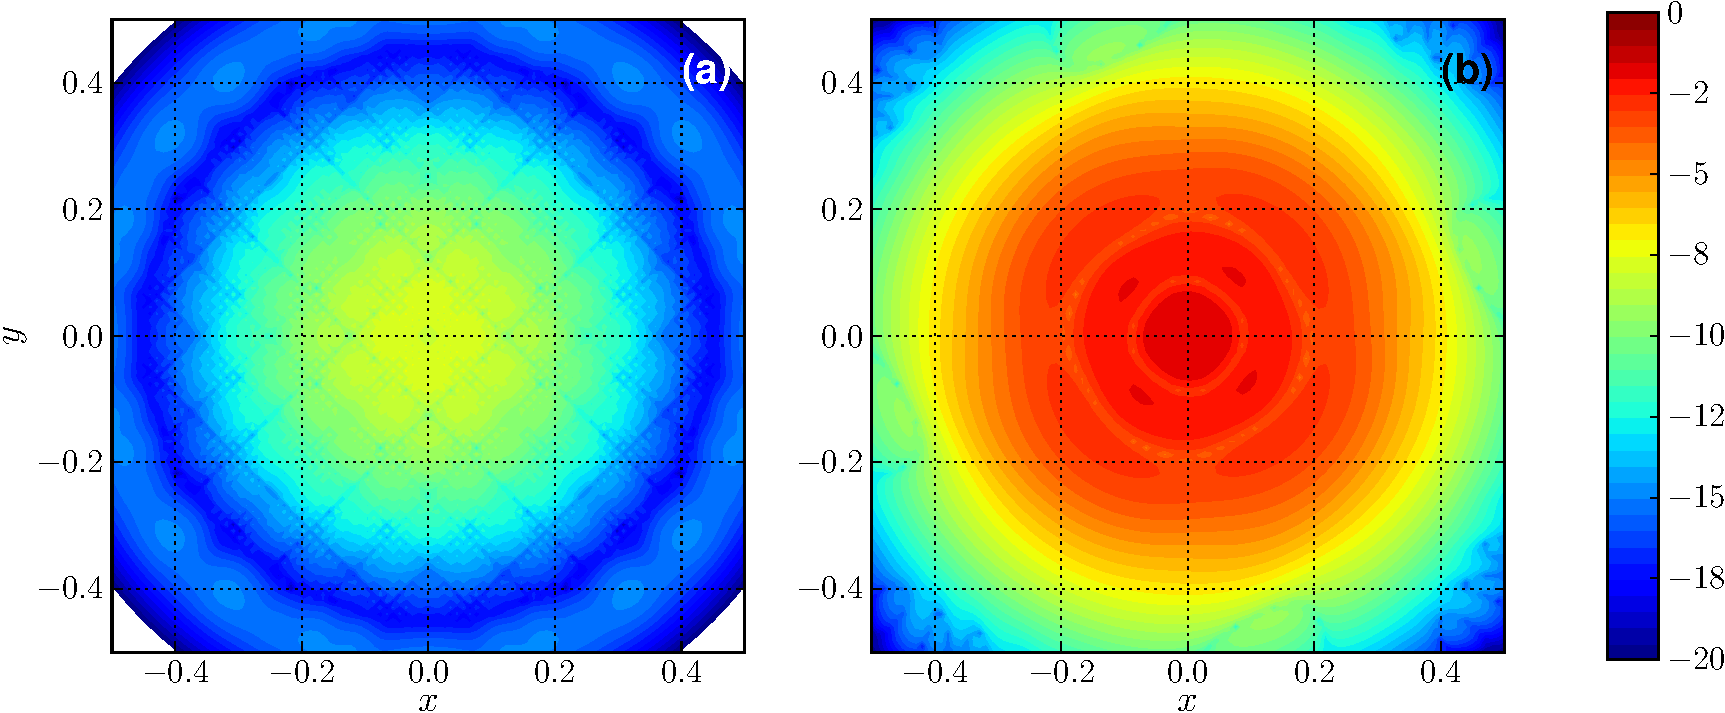
\includegraphics[width=0.99\textwidth]{figures/lagrangian/lambOseen_convection_vorticityErrorContours_compressed-crop.pdf}
	\caption{Relative error growth of Lamb-Oseen vorticity during the evolution (in logarithmic scale). The figure shows \textbf{(a)}, the initial relative error at $t_0=4$, and \textbf{(b)} the final relative error in vorticity at $t_f=5$.}
	\label{fig:lambOseen_convection_vorticityErrorContours_compressed}
	\end{figure}

	\begin{figure}[p]
	\centering
	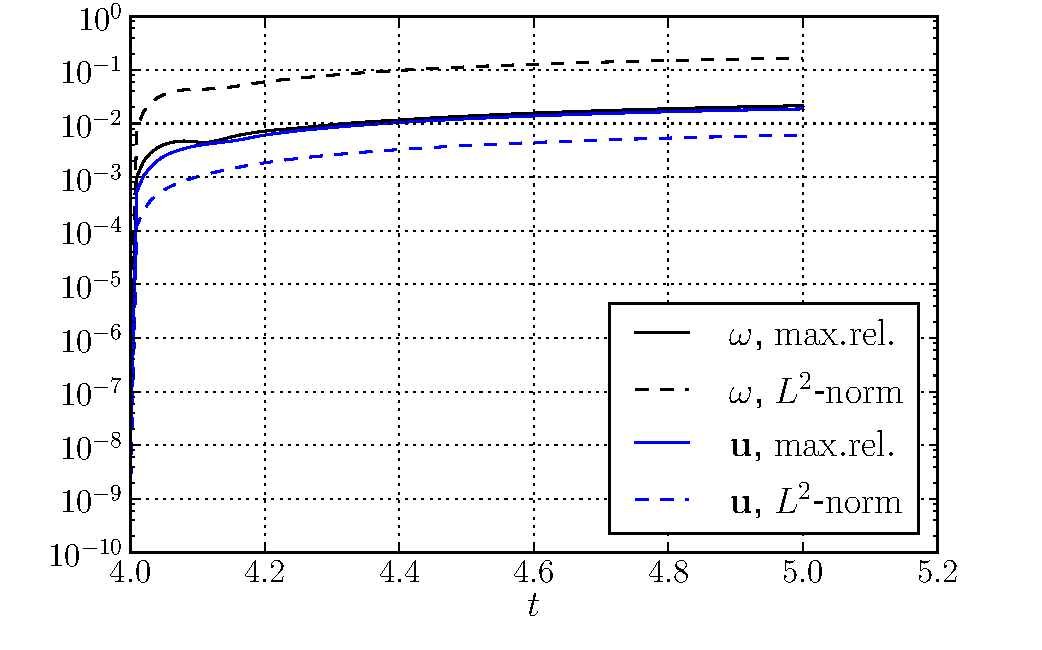
\includegraphics[width=0.7\textwidth]{figures/lagrangian/lambOseen_convection_errorGrowth_compressed.pdf}
	\caption{Relative error growth of Lamb-Oseen vortex during the evolution from $t_0=4$ to $t_f=5$. Figure depicts the error in vorticity: maximum relative error [ ---, solid black], and error in $L^2-\mathrm{norm}$ [ - -, dashed black]; and error in velocity: maximum relative error [ {\color{plotBlue}{---}}, solid blue], and error in $L^2-\mathrm{norm}$ [ {\color{plotBlue}{- -}}, dashed blue].}
	\label{fig:lambOseen_convection_errorGrowth_compressed}
	\end{figure}

So, using the Tutty's diffusion method (the simple redistribution scheme, section \ref{subsubsec:srs}), we convect and diffuse the vortex blobs with a $\Delta t_c=\Delta t_d = 0.01$. The time integration of the problem is done using a $4^{\mathrm{th}}$-order Runge-Kutta method ($\mathrm{RK4}$), ensuring accurate convection of the blobs. After the convection process, we will have to treat the Lagrangian distortion of the blobs using the remeshing scheme discussed in section \ref{subsec:remeshing}. Generally, the remeshing is typically done every 10 iterations \cite{Barba2004c}. However, as our diffusion scheme and hybrid method requires structured lattice of vortex blobs for efficient calculations, we will remesh after every step, $f_{\mathrm{redist}}=1$.  

In additional, after the evolution process, we can perform a population control on the vortex blobs to keep the simulation as efficient as possible. The \indexAcron{Population Control}{PC} removes vortex blobs that have very small circulation strengths. After the diffusion and remeshing, we will be left with vortex blobs with strengths close to numerical precision, as they have minimal impact on the accuracy of the vorticity field, we can removed them. When performing the population control, we to ensure that the loss of total circulation is at minimal. We place a tolerance on the conservation of circulation, and from literature \cite{Barba2004c}, we see that a cap of $\Gamma_{\mathrm{threshold}}=\num{1e-14}$ is acceptable. 

To verify whether our Lagrangian scheme is function according to theory, we evaluated the error growth of the simulation. Figure \ref{fig:lambOseen_convection_vorticityErrorContours_compressed}, shows the initial and the final relative error in vorticity. We see that initially we have a maximum relative error around \num{e-8}, located at the center of the Lamb-Oseen core. After 100 time integration steps from $t_0=4$ to $t_f=5$, we see that the maximum relative error in vorticity increases from \num{e-8} to \num{e-2}. The error of the vorticity are predominantly localized at the center of the core. This is because, this is where we have the highest gradient in the vorticity, as seen from figure \ref{fig:lambOseen_vorticityDistribution}. Therefore, with the current vortex blob discretization, we are not able to reconstruct this large gradient of the vorticity field. 

Figure \ref{fig:lambOseen_convection_errorGrowth_compressed}, shows the error growth of the Lamb-Oseen vortex from $t_0=4$ to $t_f=5$. The figure plots the error growth of the vorticity and the velocity. Due to the relation of the vorticity and the velocity, the error of the vorticity is an order higher that the error in the velocity. The figure shows the both the maximum relative error, and the error in the $L^2-\mathrm{norm}$. The maximum relative error (e.g. for vorticity), is determined as,
	\begin{equation}
	\left\Vert \omega^{\mathrm{exact}} - \omega^{\mathrm{discrete}} \right\Vert_{\infty} = \frac{\max\{\left|\omega^{\mathrm{exact}} - \omega^{\mathrm{discrete}}\right|\}}{\max\{\left|\omega^{\mathrm{exact}}\right|\}},
	\label{eq:maxRelErrorDef}
	\end{equation}
where $\omega^{\mathrm{exact}}$ is analytical vorticity field, and $\omega^{\mathrm{discrete}}$ is the numerical vorticity field from the vortex blobs. The error in the $L^2-\mathrm{norm}$ of the vorticity is calculated as 

	\begin{equation}
	\left\Vert \omega^{\mathrm{exact}} - \omega^{\mathrm{discrete}} \right\Vert_2 = \left(\sum_{i}^{N}\left| \omega^{\mathrm{exact}} - \omega^{\mathrm{discrete}} \right|^2 \cdot h^2\right)^{\frac{1}{2}},
	\end{equation}

and the error in velocity is calculated using the same principle. Investigating the plot, we see that after the first iteration, there is sudden increase in the error, but as time progresses the error growth stabilizes. From literature, we see that this trend has also been observed by Barba \cite{Barba2004c} and Speck \cite{Speck2011a}. For comparison, we used similar parameters, and we observe that the sudden jump in error has been similar to the literature.
	
\subsubsection*{Comparison of diffusion schemes: SRS vs. MRS}

To observe how both the diffusion scheme compare, we ran test cases with both diffusion schemes. From the simulation, we were able to observe that the Tutty's diffusion scheme, SRS, performed better that Wee's diffusion scheme, MRS. Figure \ref{fig:lambOseen_diffusionMethod_comparison_compressed} shows the error growth of maximum relative error in vorticity for both diffusion schemes. The solid lines represents the solution of the MRS and the dashed lines shows the SRS. The convection and the diffusion time steps where controlled by modifying the blob spacing $h$, and keeping the convection time step size $\Delta t_c = 0.01$. 

At $h = \num{4e-3}$, both schemes have the diffusion time step $\Delta t_d = 0.01$ meaning that the diffusion occurs at every iteration $k_d = 1$. During this time we see that the MRS performs slightly better that the SRS scheme. This is because, the diffusion of the vortex blobs is directly incorporated into the remeshing process, whereas the Tutty's SRS segregates the diffusion and the remeshing into two subsequent process. 

At $h = \num{5e-3}$, the diffusion constraint on the Wee's MRS changes the minimum allowable diffusion time step to $\Delta t_d = 0.02$, meaning that diffusion has to be performs at every second step, $k_d=2$. Whereas for Tutty's SRS, we are not constraint by the minimum diffusion time step as so we can perform diffusion at $k_d = 1$. When investigating the growth in error for MRS, we see that the diffusion scheme has a large increase in the error, whereas the SRS does not have this limitation and is still able to diffuse at every step and has only a slight increase in error, figure \ref{fig:lambOseen_diffusionMethod_comparison_compressed} (solid black line). The diffusion scheme over-estimates the diffusion, and results in an incorrect diffusion process. However, we see that Tutty's SRS still performs a stable diffusion (dashed black line).

This verification of the diffusion scheme showed that if Wee's MRS diffuses at $k_d > 1$, it will over-estimate the diffusion of the vorticity. Therefore, when using this scheme we will have to ensure that $k_d = 1$, by adjusting the convective time step appropriately. However, for large Reynolds number flows this is not possible, and so we must rely on the more stable and versatile Tutty's SRS diffusion scheme.

	\begin{figure}[!t]
	\centering
	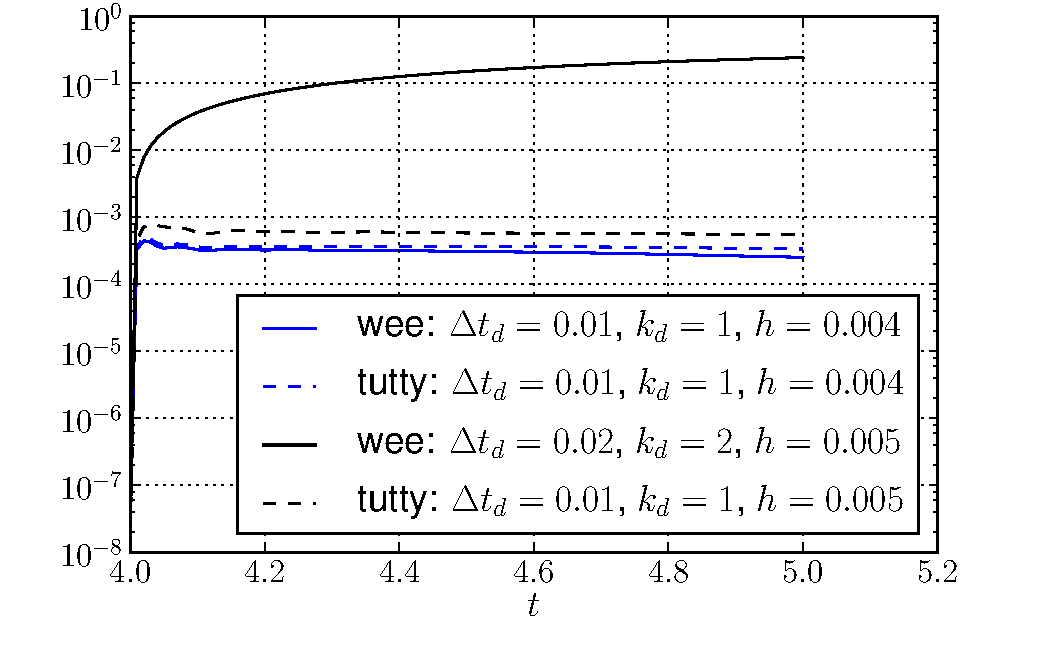
\includegraphics[width=0.7\textwidth]{figures/lagrangian/lambOseen_diffusionMethod_comparison_compressed.pdf}
	\caption{Comparison of Tutty's, simple redistribution scheme and Wee's modified interpolation method for treating diffusion. Figure depicts the growth in maximum relative error in vorticity from $t_0=4$ to $t_f=5$ at $\Delta t_c = 0.01$. The Wee diffusion scheme with $\Delta t_d = \Delta t_c = 0.01$ [{\color{plotBlue}{---}}, solid blue], and $\Delta t_d = 2 \Delta t_c = 0.02$ [---, solid black]. The Tutty's diffusion scheme, $c^2 = 1/3$, with $\Delta t_d = \Delta t_c = 0.01$ [ {\color{plotBlue}{- -}}, dashed blue], and $\Delta t_d = \Delta t_c = 0.02$ [ - -, dashed black].}
	\label{fig:lambOseen_diffusionMethod_comparison_compressed}
	\end{figure}

	\begin{figure}[p]
	        \centering
	        \begin{subfigure}[b]{0.5\textwidth}
	                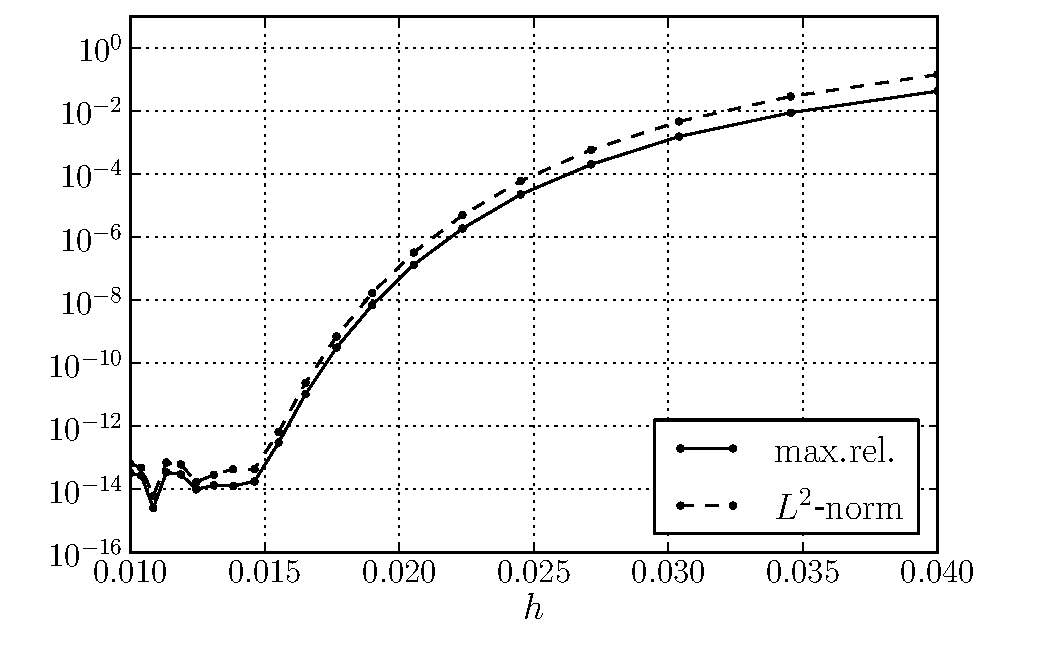
\includegraphics[width=\textwidth]{figures/lagrangian/lambOseen_convergence_dx_sigma0p02_compressed.pdf}
	                \caption{Error in vorticity vs. $h$ with $\sigma = 0.02$}
	                \label{fig:lambOseen_convergence_dx_sigma0p02_compressed}
	        \end{subfigure}%
	        ~ %add desired spacing between images, e. g. ~, \quad, \qquad etc.
	          %(or a blank line to force the subfigure onto a new line)
	        \begin{subfigure}[b]{0.5\textwidth}
	                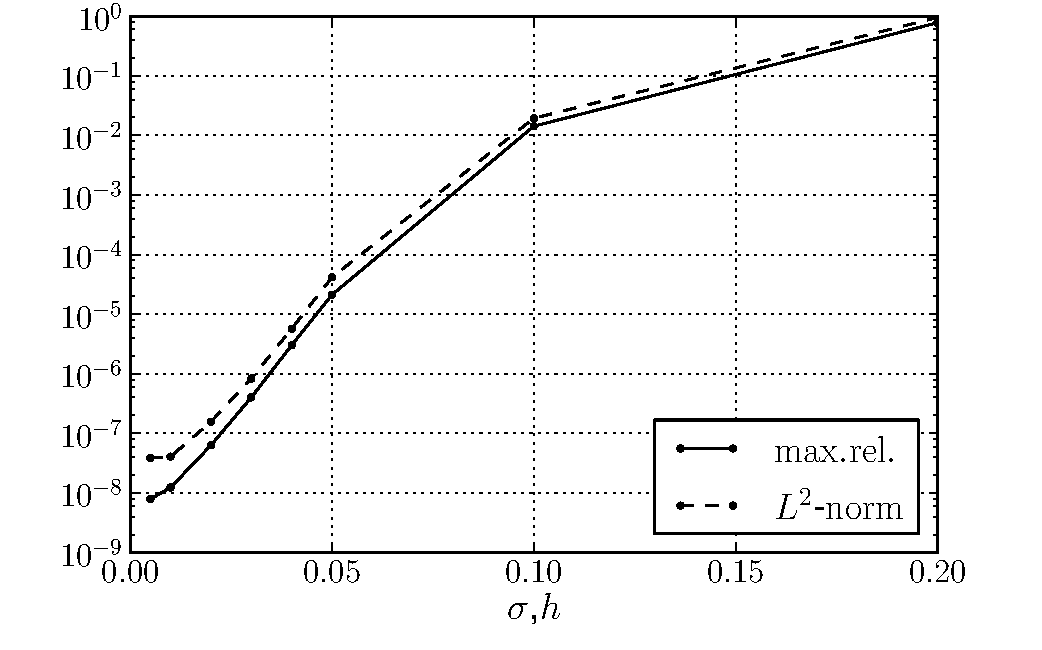
\includegraphics[width=\textwidth]{figures/lagrangian/lambOseen_convergence_dx_compressed.pdf}
	                \caption{Error in vorticity vs. $h$, $\sigma$ with $\mathrm{overlap}=1$.}
	                \label{fig:lambOseen_convergence_dx_compressed}
	        \end{subfigure}
	        \caption{Convergence in spatial discretization of the vortex blobs. Figure \textbf{(a)} shows the convergence by fixing the core size $\sigma$ and \textbf{(b)} shows the convergence when overlap ratio is fixed.}
	        \label{fig:lambOseen_convergence_dx}
	\end{figure}

	\begin{figure}[p]
	\centering
	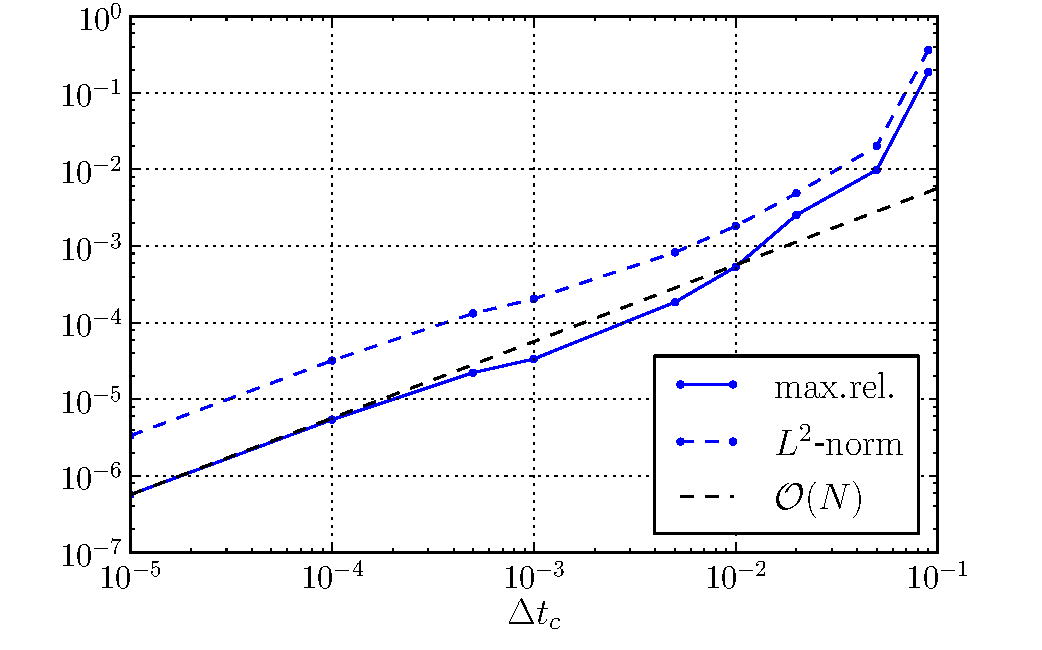
\includegraphics[width=0.6\textwidth]{figures/lagrangian/lambOseen_convergence_dt_compressed.pdf}
	\caption{Error growth of Lamb-Oseen vorticity field after one-step.}
	\label{fig:lambOseen_convergence_dt_compressed}
	\end{figure}


\subsection{Convergence study of the viscous vortex method}

Finally, we can perform a converge study, to validate that our scheme works according to the theory. For a scheme that is numerically stable, the error due to discretization must converge as the resolution of the discretization increases. 

First, we investigate the convergence in spatial discretization. As we are dealing with vortex blobs, there are multiple ways of increasing the resolution. The straight forward method would be to increase the density of particles in a given area, i.e. reducing the blob spacing $h$ and maintaining the core spreading $\sigma$. Figure \ref{fig:lambOseen_convergence_dx_sigma0p02_compressed} shows the convergence of the spatial discretization when the core size $\sigma$ is maintained at $\sigma=0.02$. At this case, the overlap ratio changes with the blob spacing, described by equation \ref{eq:overlapRatio}. At small blob spacing $h$, the error in vorticity quickly drops to near machine precision. When investigating the order of converges, we that the error converges in a non-linear fashion and similar results have been obtained by Barba \cite{Barba2004c}.

Figure \ref{fig:lambOseen_convergence_dx_compressed}, shows the convergence of error when the overlap ratio is fixed, $\mathrm{overlap} = 1$. In this test case, the core size scaled with the blob spacing, $h=\sigma$, and when increasing the spatial resolution, the error converges at non-linear fashion.
	
To investigate the convergence in temporal discretization, we determined the growth in Lamb-Oseen vorticity field after convecting with various convection step size $\Delta t_c$. Note that to perform this convergence study accurately, we had to rely on the Tutty's SRS diffusion scheme, so that $\Delta t_d = \Delta t_c$. Figure \ref{fig:lambOseen_convergence_dt_compressed} shows the convergence of the error for various temporal discretization. With the combined convection and diffusion scheme, we see that error converges at $\mathcal{O}(\Delta t)$, meaning that the vortex blobs evolution is $1^{\mathrm{st}}$-order in time.




\section{Summary of the Lagrangian method}

In summary, we have investigated the Lagrangian domain of our hybrid method in this chapter. The Lagrangian method was used to described the evolution of the wake past the geometry. \printAcron{Vortex Particle Method}{VPM} was an ideal choice to describe the wake, as we require only to evolve the wake, and the generation of the vorticity is dealt with in the Eulerian domain. Unlike the Eulerian method, VPM only required the fluid elements where there was vorticity, meaning that the VPM was inherently auto-adaptive. Using the Population Control method, we were able to remove vortex blobs where they were not needed. Furthermore, the computation of the these elements were accelerated using an FMM, and simultaneously was parallelized using a GPU hardware. 

For the VPM, the choice of fluid elements was vortex blobs. This had non-zero core size, removing the singularity when performing Biot-Savart calculations. The strengths of these particles were initialized by assigning the local circulation strength to the particle, given by equation \ref{eq:particleCirculationAssignment}. When we perform coupling, we will see that the gaussian blurring of the original vorticity field during the initialization is the fundamental source of error. Strategies such as Beale's iterative method, cannot be used as it is defined for an unbounded domain. The only approach to minimize the gaussian spreading initialization error was to increase the overlap ratio to $overlap=1$, and minimize the blob spacing $h$ as much as possible. So, the proper handling of the initialization of the vortex blob strength is still an open question, and recommend that if solved can significantly improve the accuracy and the efficiency of the hybrid coupling. More on this will be discussed in section \ref{}. \todo{citation}

The convection of the vortex blobs was done by using a $4^{\mathrm{th}}$-order Runge-Kutta time integration method. However, due to high strains in the fluid, we had to deal with the Lagrangian grid distortion of the vortex blob lattice. To deal with this, we used a $\mathrm{M}'_4$ interpolation kernel that remeshed the particles onto a structured grid.

The diffusion of the vortex blobs was also import when simulation viscous flows. Initially, we employed the modified interpolation kernel by Wee \cite{Wee2006a}, which integrated the diffusion process into the standard interpolation kernel. However, the method posed two problems: the diffusion time step $\Delta t_d$ had a lower limit; the scheme over-estimated the diffusion when the diffusion did not occur at every step, $k_d > 1$. To overcome this problem, we used the simple redistribution scheme by Tutty \cite{Tutty2010a}, which enabled us to perform diffusion after every convection step. This also ensured that the diffusion process was continuous, which was important when performing the coupling algorithm.

To deal the body boundary in the flow, we used the vortex panels to enforce the no-through/no-slip boundary condition. Koumoutsakos, Leonard, and Pepin \cite{Koumoutsakos1994b}, have shown that enforcing no-slip boundary condition is equivalent to a no-through boundary condition, as they are linked. Constant-Strength Vortex panels, based of Katz \cite{Katz2001a}, were used to treat the body boundary condition. This panel method was then verified and validated with the analytical solution of a potential flow around a cylinder. There was one difference between our vortex panel method and the standard boundary element method that is used in a typical VPM. Our panel method cannot be used to determine the vorticity generation at the body, as this is done in our Eulerian method. So we validated our Lagrangian method separately; first ensuring that the no-through boundary condition is satisfied at the vortex panels, second ensuring that the vorticity of the flow is handled properly by the vortex blobs.

To validate the vortex blob, we used the analytical solution of the Lamb-Oseen vortex problem. We verified that the Wee's MRS diffusion method indeed did not perform optimally for all parameters. The validation was done by investigating the error in the vorticity and the velocity field and was able to conclude that the vortex blobs performed according to literature of Barba \cite{Barba2004c}.

\subsection*{Lagrangian method algorithm}

	\begin{figure}[!t]
		\centering
		\begin{tikzpicture}
			[node distance=.8cm, start chain=going below,]
			\node[punktchain, join] (solvePanel) {Solve for panels};
		    \node[punktchain, join] (solveVelocity) {Evaluate the total velocity field};
		    \node[punktchain, join] (convect)     {Convect the vortex blobs};
		    \node[punktchain, join] (remesh) 	  {Remesh the Lagrangian field};
		    \node[punktchain, join] (diffuse)     {Diffuse the vortex blobs};		    
		\end{tikzpicture}
		\caption{Flowchart of the Lagrangian method. The flowchart shows coupling between vortex panels and vortex blobs to evolve from $t_n$ to $t_{n+1}$.}
		\label{fig:flowchart_lagrangian}
	\end{figure}
	
The flowchart to one time step of the Lagrangian method is given by figure \ref{fig:flowchart_lagrangian}.The algorithm to the Lagrangian method can be summarized as follows:
	\begin{enumerate}
	\item \textbf{Solve for panels:} Determine the strengths of the vortex panels $\gamma$, such that the no-slip boundary condition at the collocation points of the vortex panels is enforced. When determining the strengths, we also have to ensure that the total circulation of the vortex panels satisfied the conservation of circulation, equation \ref{eq:circulationNet}.
	\item \textbf{Evaluate the total velocity field:} Evaluate the total velocity field $\mathbf{u}$, which is the sum of velocity field induced by the vortex blobs $\mathbf{u}_{\omega}$, the velocity field induced by the vortex panels $\mathbf{u}_{\gamma}$, and the free-stream velocity field $\mathbf{u}_{\infty}$. 
	\item \textbf{Convect the vortex blobs:} Use the velocity field to time step the vortex blobs from $t_n$ to $t_{n+1}$ to the new position with a convection time step $\Delta t_c$.
	\item \textbf{Remesh the Lagrangian field:} Remesh the vortex blobs onto a structured square lattices using the $\mathrm{M}'_4$ interpolation kernel.
	\item \textbf{Diffuse the vortex blobs:} Diffuse the vortex blobs using the $\Delta t_d$ diffusion time step, by modifying the strengths of the vortex blobs according to Wee's MRS or Tutty's SRS method.
	\end{enumerate}

The generation of the vorticity is dealt with in the Eulerian domain, which is explained in chapter \ref{ch:eulerian}. The vorticity is then transfered into the Lagrangian domain using the Hybrid coupling scheme, which was summarized in the introduction, chapter \ref{ch:introduction}, and full elaborated in chapter \ref{ch:hybrid}.
s
\section{Chapter Nomenclature}

{\textbf{\textsf{Latin Symbols}}}

{\renewcommand{\arraystretch}{1.2} %<- modify value to suit your needs
\begin{longtable}{p{1.5cm}p{10.5cm}p{1.5cm}}
    $\mathbf{A}$			& Vortex panel influence matrix						& -\\         

	$c^2$ 					& Diffusion parameter 								& - \\

    $\mathcal{E}$			& Enstrophy			  								& \si{m^2.s^{-2}} \\

    $h$						& Nominal particle spacing							& \si{m}\\   
    $h_{\nu}$				& Characteristic diffusion distance					& \si{m}\\ 

	$k_d$ & Frequency of vortex blob diffusion  								& -\\
    $\mathbf{K}$			& Biot-Savart kernel 								& -\\ 
    $\mathbf{K}_{\sigma}$	& Vortex blob kernel 								& -\\     

	$\hat{\mathbf{n}}$  	& Unit normal vector 								& -\\
	$N$  					& Number of vortex blobs (particles) 				& -\\

	$\mathrm{Ov}$			& Overlap ratio 									& - \\    
	
	$p$						& Pressure											& \si{Pa}\\

	$r$ 					& Radial position 									& \si{m}\\
	
	$\hat{\mathbf{s}}$		& Unit tangent vector								& - \\
	
	$t$						& Simulation time									& \si{s} \\
	
	$\mathbf{u}$			& Velocity 											& \si{m.s^{-1}}\\
	$\mathbf{u}_b$			& Velocity of the body 								& \si{m.s^{-1}}\\
	$\mathbf{u}_{\gamma}$	& Vortex sheet induced velocity                   	& \si{m.s^{-1}}\\	
	$\mathbf{u}_{\mathrm{ext}}$		& External induced velocity							& \si{m.s^{-1}}\\	
	$\mathbf{u}^h$			& Discrete velocity                               	& \si{m.s^{-1}}\\		
	$\mathbf{u}_{\infty}$	& Free-stream velocity								& \si{m.s^{-1}}\\			
	$\mathbf{u}_{\phi}$		& Free-stream velocity                            	& \si{m.s^{-1}}\\				
	$u_{r}$					& Radial velocity									& \si{m.s^{-1}}\\			
	$u_{\theta}$			& Angular velocity                               	& \si{m.s^{-1}}\\
	$\mathbf{u}_{\mathrm{slip}}$	& Boundary slip velocity					& \si{m.s^{-1}}\\
	$\mathbf{u}_{\omega}$	& Vorticity velocity 								& \si{m.s^{-1}}\\	

	$W$ 					& Interpolation kernel weight 						&-\\		
	$\mathbf{x}$			& Position vector 									& \si{m}\\		
	$\mathbf{x}_{\nu}$		& Position vector of particle to be diffused 		& \si{m}\\			
	$\mathbf{x}_{p}$		& Position vector of vortex blob (particle)			& \si{m}\\				
    %\caption{Attributes of \texttt{HybridSolver} class and their description.}
    %\label{tab:attributeHybrid}
\end{longtable}}

{\textbf{\textsf{Greek Symbols}}}

{\renewcommand{\arraystretch}{1.2} %<- modify value to suit your needs
\begin{longtable}{p{1.5cm}p{10.5cm}p{1.5cm}}
	$\alpha_p$ 		& Circulation of the particle & \si{m^2.s^{-1}}\\
	$\beta_p$ 		& Corrected circulation of the particle & \si{m^2.s^{-1}}\\	

	$\Delta t_c$ 		& Convection time step size & \si{s}\\
	$\Delta t_d$ 		& Diffusion time step size & \si{s}\\	

	$\epsilon$ 		& Relative error & -\\		

	$\Gamma$ 		& Circulation & \si{m^2.s^{-1}}\\	
	$\Gamma_b$ 		& Circulation inside a moving body & \si{m^2.s^{-1}}\\		
	$\gamma_c$ 		& Vortex sheet strength & \si{m^2.s^{-1}}\\			
	$\gamma_{\gamma}$ 	& Circulation of the vortex sheet & \si{m^2.s^{-1}}\\				
	$\gamma_{\omega}$ 	& Circulation of the fluid & \si{m^2.s^{-1}}\\					

	$\nu$ & Kinematic viscosity & \si{m^2.s^{-1}}\\

	$\omega$ & Vorticity & \si{s^{-1}}\\
	$\tilde{\omega}$ & Vortex blob cell vorticity & \si{s^{-1}}\\
	$\omega^h$ & Discrete vorticity field & \si{s^{-1}}\\

	$\rho$ & Density & \si{kg.m^{-3}}\\
	
	$\sigma$ & Core size & \si{m}\\
	$\tau$ & Scaled viscous time & \si{m^2}\\
	$\xi$ & Scale relative position of particle to stencil node & -\\
	$\zeta_{\sigma}$		& Smooth cut-off function of the blobs & -\\			

\end{longtable}}

